\documentclass[12pt, letterpaper]{article}
\usepackage[margin=1 in]{geometry}
\usepackage[mathscr]{euscript}
\usepackage{amsfonts}
\usepackage{amsmath}
\usepackage{amssymb}
\usepackage{graphicx}
\usepackage{parskip}
\usepackage{minted} 
\setminted[Python]{
    frame=lines,
    framesep=2mm,
    baselinestretch=1.2,
    bgcolor=LightGray
}
\usepackage{xcolor} % to access the named colour LightGray
\definecolor{LightGray}{gray}{0.9}
\usepackage{listings}% http://ctan.org/pkg/listings
\lstset{
  basicstyle=\ttfamily,
  mathescape
}
\graphicspath{{./images/}}
\setlength{\parindent}{0pt}
\newcommand{\R}{\mathbb{R}}
\newcommand{\mdash}{
\draw(0.3,0.5ex)--(-0.3,0.5ex);
}

\title{Deep Learning Specialization}
\author{Declan Lim}

\begin{document}
    \maketitle
    \pagebreak

    \section{Neural Networks and Deep Learning}
    \subsection{Introduction to Deep Learning}
    \begin{itemize}
        \item Takes input $x$ to a ``neuron'' and gives some output $y$   
        \begin{figure}[ht]
            \centering
            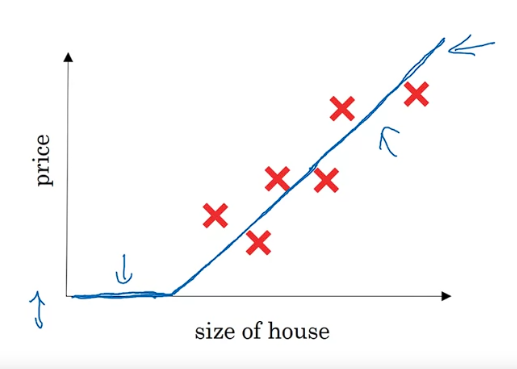
\includegraphics[width=8cm]{1.png}
        \end{figure}
        \begin{itemize}
            \item Simple neural network has a single input, neuron and output
            \item $x$: size of the house
            \item $y$: price of the house
            \item Hypothesis (blue line) is a ReLU (Rectified Linear Unit)
        \end{itemize}
        \item More complex neural networks can be formed by ``stacking'' neurons
        \begin{figure}[ht]
            \centering
            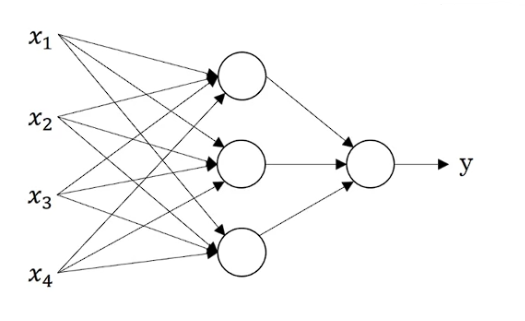
\includegraphics[width=8cm]{2.png}
        \end{figure}
        \item Every input layer feature is interconnected with every hidden layer feature
        \begin{itemize}
            \item The neural network will decide what the intermediate features will be
        \end{itemize}
        \item Most useful in supervised learning settings
    \end{itemize}
    \hspace{3mm}
    \subsubsection{Supervised Learning}
    \begin{itemize}
        \item Aims to learn a function to map an input $x$ to an output $y$
        \begin{itemize}
            \item Real estate: predicting house prices from the house features
            \item Online advertising: showing ads based on probability of user clicking on ad
            \item Photo tagging: tagging images based on objects in the image
            \item Speech recognition: generating a text transcript from audio
            \item Machine translation: translating from one language to another
            \item Autonomous driving: returning the positions of other cars from images and radar info
        \end{itemize}
        \item Different types of neural network used for different tasks
        \begin{itemize}
            \item Standard neural network: real estate and online advertising
            \item Convolutional neural network (CNN): image data
            \item Recurrent neural network (RNN): audio and language data (sequenced data)
            \item Hybrid neural network: Autonomous driving (more complex input)
        \end{itemize}
        \begin{figure}[ht]
            \centering
            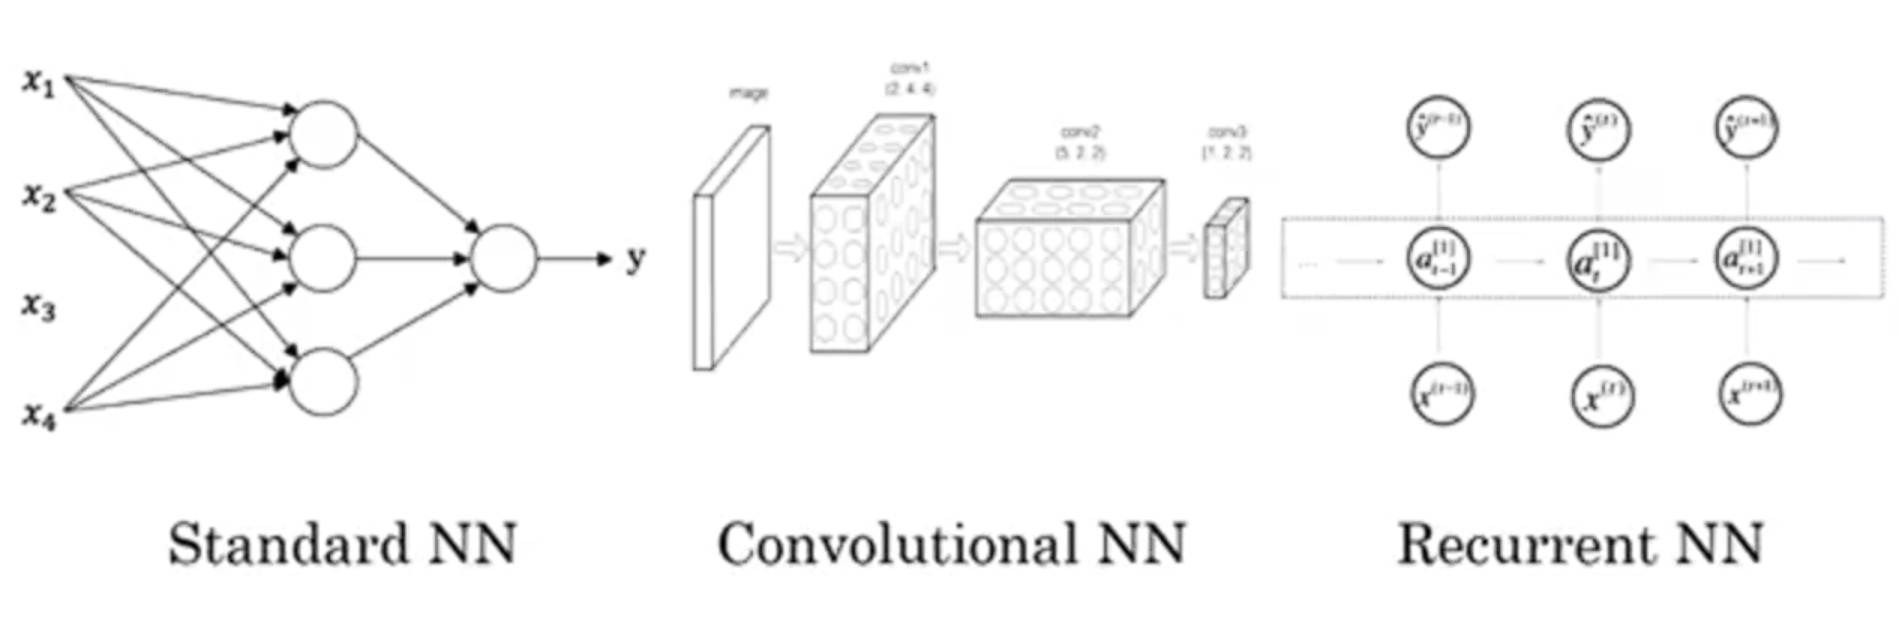
\includegraphics[width=10cm]{3.png}
        \end{figure}
        \item Supervised learning can be applied to structured and unstructured data
        \begin{itemize}
            \item Structured data has features with well defined meanings 
            \item Unstructured data has more abstract features (images, audio, text)
        \end{itemize}
    \end{itemize}

    \hspace{30mm}
    \begin{itemize}
        \item Deep learning has only recently started to become more widespread
        \begin{itemize}
            \item Given large amounts of data and a large NN, deep learning will outperform more traditional learning algorithms
            \item For small amounts of data, any performance of the algorithm depends on specific implementation
        \end{itemize}
        \begin{figure}[ht]
            \centering
            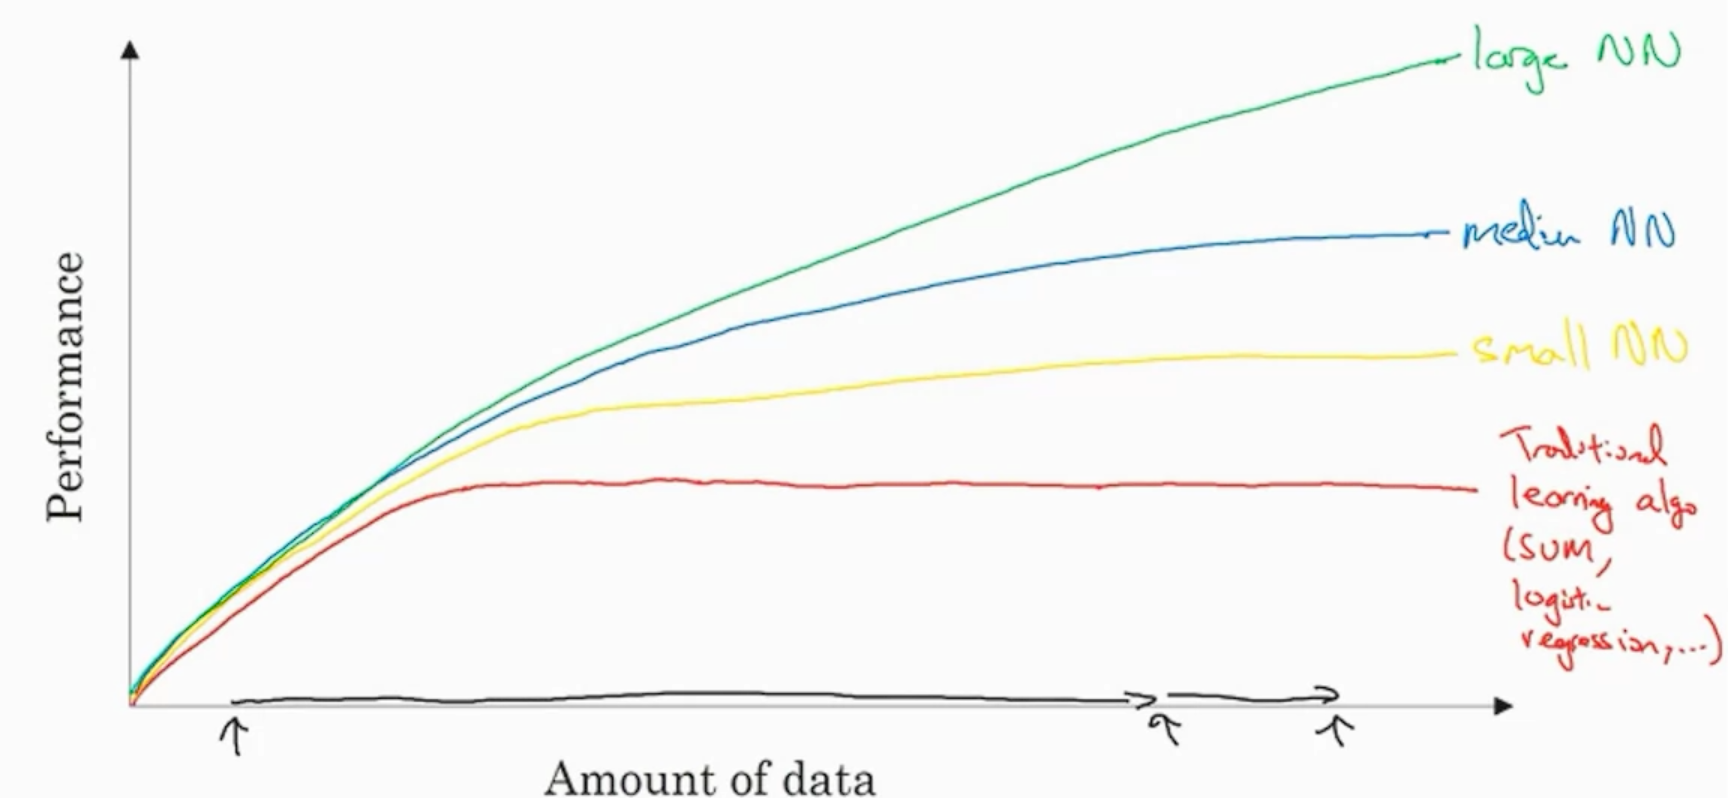
\includegraphics[width=8cm]{4.png}
        \end{figure}
        \item ``Scale drives deep learning progress''
        \begin{itemize}
            \item Both the scale of the data and the NN
        \end{itemize}
        \item Recent algorithmic innovations with increase scale of computation
        \begin{itemize}
            \item Idea to switch from sigmoid activation function to ReLu function increased NN performance
            \item Ends of sigmoid function have close to 0 gradient so and therefore result in small changes in $\theta$
            \item ReLu function has gradient of 1 for positive values
        \end{itemize}
        \item Neural network process is iterative
        \begin{itemize}
            \item Increasing speed at which a NN can be trained allows different ideas to be tried
        \end{itemize}
    \end{itemize}
    \subsection{Neural Network Basics}
    \subsubsection{Logistic Regression as a Neural Network}
    \begin{itemize}
        \item Logistic regression used for binary classification
        \item For a colour image, of 64$\times$64 pixels, will have total 12288 input features
        \begin{itemize}
            \item Image is stored as 3 separate matrices for each colour channel
            \item All pixel intensities should be unrolled into a single feature vector
            $$n=12288$$
            $$x\in\R^{12288}$$
            \item For a matrix \texttt{X} of shape $(a,b,c,d)$, want a matrix \texttt{X\_flatten} of shape $(b*c*d,1)$
        \end{itemize}
        \begin{minted}{Python}
            X_flatten = X.reshape(X.shape[0], -1).T
        \end{minted}
        
    \end{itemize}
    
    \vspace{5mm}
    \textbf{Notation} 
    $$\{(x^{(1)},y^{(1)}),(x^{(2)},y^{(2)}),...,(x^{(m)},y^{(m)})\}$$
    \begin{itemize}
        \item $(x,y)$: single training example
        \begin{itemize}
            \item $x\in\R^{n_x}$ ($n_x=$ number of features)
            \item $y\in\{0,1\}$
        \end{itemize}
        \item $(x^{(i)},y^{(i)})$: $i^{th}$ training example
        \item $m=m_{train}$
        \item $m_{test}=$ \# of test examples
        \item $X=\begin{bmatrix}
            \mid & \mid & & \mid \\
            x^{(1)} & x^{(2)} & ... & x^{(3)} \\
            \mid & \mid & & \mid \\
        \end{bmatrix}$
        \begin{itemize}
            \item $X\in\R^{n_x\times n}$
        \end{itemize}
        \item $Y=\begin{bmatrix}
            y^{(1)} & y^{(2)} & ... & y^{(m)}
        \end{bmatrix}$
        \begin{itemize}
            \item $Y\in\R^{1\times m}$
        \end{itemize}
    \end{itemize}

    \vspace{5mm}
    \textbf{Logistic Regression}
    \begin{itemize}
        \item Given $x$, want $\hat{y}=P(y=1|x)$
        \begin{itemize}
            \item Since $\hat{y}$ is a probability, want $0\leq\hat{y}\leq1$
        \end{itemize}
        \item Parameters: $w\in\R^{n_x}, b\in\R$
        \item Output: $\hat{y}=\sigma(w^Tx+b)$
        \begin{figure}[ht]
            \centering
            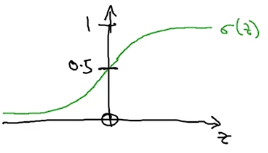
\includegraphics[width=8cm]{5.png}
        \end{figure}
        $$\sigma(z)=\frac{1}{1+e^{-z}}$$
        $$z=w^Tx+b$$
        \item Aim is to learn parameters $w$ and $b$ such that $\hat{y}$ is a good estimate of the probability
        \item Previous convention had $\theta$ vector with an additional $\theta_0$ parameter
        \begin{itemize}
            \item Keeping $\theta_0$ ($b$) separate from the rest of the parameters is easier to implement
        \end{itemize}
    \end{itemize}

    \vspace{3mm}
    \textbf{\textit{Cost Function}}
    \begin{itemize}
        \item Given $\{(x^{(1)}, y^{(1)}),(x^{(2)}, y^{(2)}), ..., (x^{(m)}, y^{(m)})\}$, want $\hat{y}^{(i)} \approx y^{(i)}$
        \item Squared error function not used for logistic regression loss function 
        \begin{itemize}
            \item Optimization problem becomes non convex and will have local optima
        \end{itemize}

        \vspace{10mm}
        $$\mathcal{L}(\hat{y},y)=-(y\log(\hat{y})+(1-y)\log(1-\hat{y}))$$
        \item If $y=1$:
        \begin{itemize}
            \item $\mathcal{L}(\hat{y},y)=-\log(\hat{y})$
            \item Want large $\log(\hat{y})$ $\therefore$ want large $\hat{y}$
            \item $\hat{y}$ has a max of 1 $\therefore$ want $\hat{y}=1$
        \end{itemize}
        \item If $y=0$:
        \begin{itemize}
            \item $\mathcal{L}(\hat{y}, y)=-log(1-\hat{y})$
            \item Want large $\log(1-\hat{y})$ $\therefore$ want small $\hat{y}$
            \item $\hat{y}$ has a min of 0 $\therefore$ want $\hat{y}=0$
        \end{itemize}
        \item Cost function:
        \begin{align*}
            J(w,b)&=\frac{1}{m}\sum_{i=1}^{m}\mathcal{L}(\hat{y}^{(i)},y^{(i)}) \\
            &= -\frac{1}{m}\sum_{i=1}^{m}[y^{(i)}\log(\hat{y}^{(i)})+(1-y^{(i)})\log(1-\hat{y}^{(i)})]
        \end{align*}
        \begin{itemize}
            \item Average loss function over all training examples
        \end{itemize}
    \end{itemize}

    \vspace{3mm}
    \textbf{\textit{Gradient Descent}}
    \begin{itemize}
        \item Want to find values of $w$ and $b$ that minimize the cost function $J(w,b)$
        \begin{itemize}
            \item For logistic regression, $w$ and $b$ usually initialized to 0
        \end{itemize} 
        \item One iteration of gradient descent will take a step in the direction of steepest descent
    \end{itemize}

    \vspace{3mm}
    \begin{lstlisting}
    Repeat {
        w := w - $\alpha \frac{\partial J(w,b)}{\partial w}$
        b := b - $\alpha \frac{\partial J(w,b)}{\partial b}$
    }  
    \end{lstlisting}
    \begin{itemize}
        \item Using the computation graph:
        \begin{figure}[ht]
            \centering
            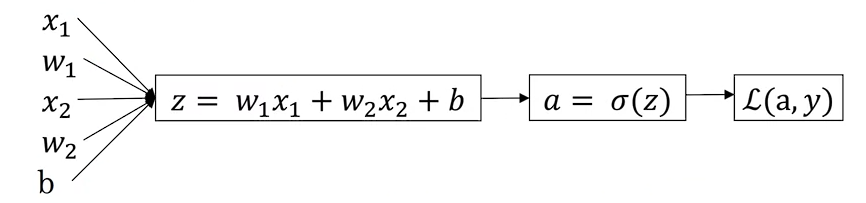
\includegraphics[width=12cm]{6.png}
        \end{figure}
        \begin{center}
            $$\frac{\partial \mathcal{L}(a,y)}{\partial a}=-\frac{y}{a}+\frac{1-y}{1-a}$$
            \begin{align*}
                \frac{\partial\mathcal{L}(a,y)}{\partial z} &=\frac{\partial\mathcal{L}}{\partial a} \times \frac{\partial a}{\partial z} \\
                &= (-\frac{y}{a}+\frac{1-y}{1-a}) \times a(1-a) \\
                &= a-y
            \end{align*}
            $$\frac{\partial\mathcal{L}}{\partial w_1}=x_1 \times \frac{\partial\mathcal{L}}{\partial z}$$
            $$\frac{\partial\mathcal{L}}{\partial w_2}=x_2 \times \frac{\partial\mathcal{L}}{\partial z}$$
            $$\frac{\partial\mathcal{L}}{\partial b}=\frac{\partial\mathcal{L}}{\partial z}$$
        \end{center}
        \item Partial derivative over all training examples calculated by taking the average \texttt{dw1}
        $$\frac{\partial}{\partial w_1}J(w,b)=\frac{1}{m}\sum^m_{i=1}\frac{\partial}{\partial w_1} \mathcal{L}(a^{(i)},y^{(i)})$$

        Initialize \texttt{J = 0, dw1 = 0, dw2 = 0, db = 0}
        \begin{lstlisting}
        For i = 1 to m:
            z$^{(i)}$ = w$^T$x$^{(i)}$ + b
            a$^{(i)}$ = $\sigma$(z$^{(i)}$)

            J += -[y$^{(i)}$ $\log$(a$^{(i)}$) + (1-y$^{(i)}$)$\log$(1-a$^{(i)}$)]
            dz$^{(i)}$ = a$^{(i)}$ - y$^{(i)}$
            dw1 += x$_1^{(i)}$ dz$^{(i)}$
            dw2 += x$_2^{(i)}$ dz$^{(i)}$
            db += dz$^{(i)}$

        J /= m
        dw1 /= m
        dw2 /= m
        db /= m

        w1 := w1 - $\alpha$ dw1
        w2 := w2 - $\alpha$ dw2 
        b := b - $\alpha$ db
        \end{lstlisting}
        \item Above implementation requires \texttt{for} loop over all features for all training examples
        \begin{itemize}
            \item Vectorization can be used to remove explicit \texttt{for} loops
            \item Vectorization required for deep learning to be efficient
        \end{itemize}
    \end{itemize}

    \subsubsection{Vectorisation in Python}
    \begin{itemize}
        \item Deep learning performs best on large data sets
        \begin{itemize}
            \item Code must be able to run quickly to be effective on large data sets
        \end{itemize}
        $$z=w^Tx + b$$
        $$w\in \R^{n_x} ~~ x\in \R^{n_x}$$
        \item Non vectorized implementation:
        \begin{minted}{Python}
            z = 0
            for i in range(n_x):
                z += w[i] * x[i]
            z += b
        \end{minted}
        \item GPUs and CPUs both have parallelization instructions (SIMD: Single Instruction Multiple Data)
        \begin{itemize}
            \item If built in functions are used, \texttt{numpy} will use parallelism to perform computations faster 
        \end{itemize}
        \item For logistic regression, need to calculate $z$ and $a$ values for each training example
        $$z^{(i)}=w^Tx^{(i)}+b$$
        $$a^{(i)}=\sigma(z^{(i)})$$
        $$X = \begin{bmatrix}
            \mid & \mid & & \mid \\
            x^{(1)} & x^{(2)} & ... & x^{(m)} \\
            \mid & \mid & & \mid 
        \end{bmatrix} $$
        $$w\in\R^{n_x} ~~ X\in\R^{n_x\times m}$$ 
        \begin{align*}
            \begin{bmatrix}
                z^{(1)} & z^{(2)} & ... & z^{(m)}
            \end{bmatrix}
            &= w^TX + \begin{bmatrix}
                b & b & ... & b
            \end{bmatrix} \\
            &= \begin{bmatrix}
                w^Tx^{(1)}+b & w^Tx^{(2)}+b & ... & w^Tx^{(m)}+b 
            \end{bmatrix}
        \end{align*}
        \item In Python:
        \begin{minted}{Python}
            Z = np.dot(w.T, X) + b
        \end{minted}
        \begin{itemize}
            \item Python will broadcast the value \texttt{b} so it can be added to the matrix
        \end{itemize}
        \item Vectorized implementation of sigmoid function can be used on \texttt{Z} to calculate \texttt{A}
        $$A= \begin{bmatrix}
            a^{(1)} & a^{(2)} & ... & a^{(m)}
        \end{bmatrix} $$
        
        $$dz^{(i)}=a^{(i)}-y^{(i)}$$
        $$dz=A-Y$$
        $$db=\frac{1}{m}\sum^m_{i=1}dz^{(i)}$$
        $$dw=\frac{1}{m}X(dz)^T$$
        \begin{minted}{Python}
            Z = np.dot(w.T,X) + b
            A = sigmoid(Z)
            dz = A - Y
            dw = 1/m * np.dot(X, dz.T)
            db = 1/m * np.sum(dz)

            # Gradient descent update
            w = w - alpha * dw
            b = b - alpha * db
        \end{minted}
        \item \texttt{for} loop is required to run multiple iterations of gradient descent
    \end{itemize}
    \subsection{Shallow Neural Networks}
    \begin{itemize}
        \item A neural network will have stacked logistic regression units in each layer
        \begin{itemize}
            \item Logistic regression output from one layer will be fed to another layer
        \end{itemize}
    \end{itemize}

    \vspace{25mm}
    \begin{itemize}
        \begin{figure}[ht]
            \centering
            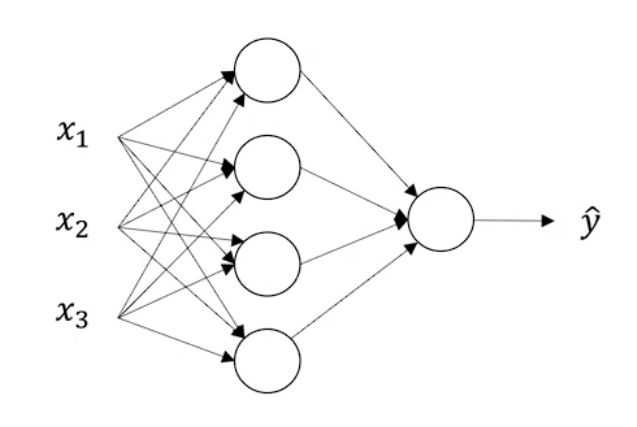
\includegraphics[width=8cm]{7.png}
        \end{figure}
        \item Input layer of the neural network contains the feature $x_1, x_2, x_3$
        \begin{itemize}
            \item $a^{[0]}=X$    
        \end{itemize}
        \item Intermediate layers in the network are hidden layers
        \begin{itemize}
            \item Hidden layers do not have ``true'' values in the training set
        \end{itemize}
        \item Final layer in the network is the output layer
        \begin{itemize}
            \item Generates the predicted value $\hat{y}$
        \end{itemize}
        \item Above diagram is a 2 layer NN
        \begin{itemize}
            \item Input layer is layer 0
        \end{itemize}
        \item Each layer will have parameters $w$ and $b$ associated with them 
        \item Each node in the NN will perform logistic regression with its inputs
        $$z_i^{[l]}=w_i^{[l]T}x+b_i^{[l]} ~~\rightarrow~~ a_i^{[l]}=\sigma(z_i^{[l]})$$
      

        $$W^{[1]} = \begin{bmatrix}
            - & w_1^{[1]T} & - \\
            - & w_2^{[1]T} & - \\
            - & w_3^{[1]T} & - \\
            - & w_4^{[1]T} & - 
        \end{bmatrix} $$
        $$a^{[0]}=\begin{bmatrix}
            x_1 \\
            x_2 \\
            x_3
        \end{bmatrix} $$
        $$b^{[1]}=\begin{bmatrix}
            b_1^{[1]} \\
            b_2^{[1]} \\
            b_3^{[1]} \\
            b_4^{[1]} 
        \end{bmatrix}$$

        \begin{align*}
            z^{[1]}&=\begin{bmatrix}
                z_1^{[1]} \\
                z_2^{[1]} \\
                z_3^{[1]} \\
                z_4^{[1]} \\
            \end{bmatrix} \\
            &= \begin{bmatrix}
                w_1^{[1]T}a^{[0]}+b_1^{[1]} \\
                w_2^{[1]T}a^{[0]}+b_1^{[1]} \\
                w_3^{[1]T}a^{[0]}+b_1^{[1]} \\
                w_4^{[1]T}a^{[0]}+b_1^{[1]} \\
            \end{bmatrix} \\
            &= w^{[1]} a^{[0]} + b^{[1]}
        \end{align*}

        \begin{align*}
            a^{[1]}&=\begin{bmatrix}
                a_1^{[1]} \\
                a_2^{[1]} \\
                a_3^{[1]} \\
                a_4^{[1]} \\
            \end{bmatrix} \\
            &= \sigma(z^{[1]})
        \end{align*}
        $$z^{[2]}=W^{[2]}a^{[1]}+b^{[2]} ~~\rightarrow~~ a^{[2]}=\sigma(z^{[2]})$$
    \end{itemize}

    \begin{itemize}
        \item Vectorized method should be able to work on all training examples at one time
        \begin{itemize}
            \item Vector for each training example can be stacked horizontally in a matrix
            \item Vertical dimension will be the number of units in a layer ($n_x$ for the input layer)
        \end{itemize}
    \end{itemize}

    $$X=\begin{bmatrix}
        \mid & \mid & & \mid \\
        x^{(1)} & x^{(2)} & & x^{(m)} \\
        \mid & \mid & & \mid
    \end{bmatrix}$$

    $$Z^{[1]}=\begin{bmatrix}
        \mid & \mid & & \mid \\
        z^{[1](1)} & z^{[1](2)} & ... & z^{[1](m)} \\
        \mid & \mid & & \mid
    \end{bmatrix}$$

    $$A^{[1]}=\begin{bmatrix}
        \mid & \mid & & \mid \\
        a^{[1](1)} & a^{[1](2)} & ... & a^{[1](m)} \\
        \mid & \mid & & \mid
    \end{bmatrix}$$
    
    \begin{align*}
        Z^{[1]}&=W^{[1]}X+b^{[1]} \\
        A^{[1]}&=\sigma(Z^{[1]}) \\
        Z^{[2]}&=W^{[2]}A^{[1]}+b^{[2]} \\
        A^{[2]}&=\sigma(Z^{[2]})
    \end{align*}

    \subsubsection{Activation Functions}
    \begin{itemize}
        \item After $z$ values are calculated, activation function must be run to get the activation value $a$
        $$a_{sigmoid}=\frac{1}{1+e^{-z}}$$
        \item Alternatively $a^{[1]}=g(z^{[1]})$ where $g$ is a non linear function
        \item $\tanh$ function almost always performs better than the sigmoid function
        \begin{itemize}
            \item Equivalent to a transformed version of the sigmoid function  
            \item $\tanh$ function is odd and is ``centered'' around the origin
            \item The mean of the data will be closer to 0 and will help with learning in the next layer
        \end{itemize}
        $$a_{\tanh}=\frac{e^z-e^{-z}}{e^z+e^{-z}}$$
        \begin{figure}[ht]
            \centering
            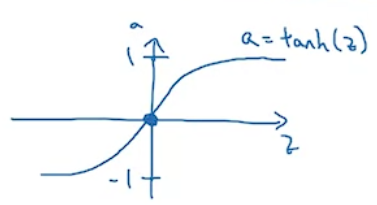
\includegraphics[width=8cm]{8.png}
        \end{figure}
        \item For binary classification, the final output layer can use the sigmoid function
        \begin{itemize}
            \item Want the value of $\hat{y}$ to be between 0 and 1
        \end{itemize}
        \item For both the sigmoid and $\tanh$ functions, when $z$ is large, the gradient is very small
        \begin{itemize}
            \item Results in a slower gradient descent
        \end{itemize}
        \item ReLU function has a gradient of 1 when $z$ is positive
        \begin{figure}[ht]
            \centering
            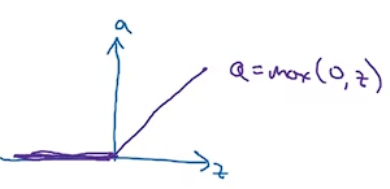
\includegraphics[width=8cm]{9.png}
        \end{figure}
        \begin{itemize}
            \item Gradient is 0 when $z$ is negative
        \end{itemize}
        \item For majority of the ReLU function, gradient is very different from 0
        \begin{itemize}
            \item Will typically allow NN to learn much faster than sigmoid or $\tanh$ function
        \end{itemize}
        \item ReLU function should be used as the default activation function
        \item The leaky ReLu function has a slight positive gradient when $z$ is negative
        $$a_{leaky ReLU}=\max(0.01z, z)$$
        \begin{figure}[ht]
            \centering
            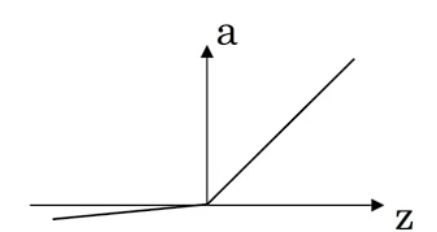
\includegraphics[width=8cm]{10.png}
        \end{figure}
        \item For a NN to compute more complex functions, activation function must be non linear
        \begin{itemize}
            \item If a linear activation function is used, final output of the NN can only be a linear function 
            \item Multiple linear activation neurons with a sigmoid as the output neuron is equivalent to standard logistic regression
        \end{itemize}
        \item Linear activation function can be used in the output layer if output is a real number
        \item Derivative of the activation function must be calculated for backpropagation
        \begin{itemize}
            \item Sigmoid function
            $$g(z)=\frac{1}{1+e^{-z}}$$
            \begin{align*}
                \frac{d}{dz}g(z)&=\frac{1}{1+e^{-z}}\left(1-\frac{1}{1+e^{-z}}\right) \\
                &=g(z)(1-g(z))
            \end{align*}
            \item $\tanh$ function
            \begin{align*}
            g(z)&=\tanh(z) \\
            &=\frac{e^z-e^{-z}}{e^z+e^{-z}}
            \end{align*}
            \begin{align*}
                \frac{d}{dz}g(z)&=1-\left(\frac{e^z-e^{-z}}{e^z+e^{-z}}\right)^2 \\
                &=1-g(z)^2
            \end{align*}
            \item ReLU function
            $$g(z)=\max(0,z)$$
            $$\frac{d}{dz}g(z)=\begin{cases}
                0 & \text{if } z < 0 \\
                1 & \text{if } z \geq 0
            \end{cases}$$
            \item Leaky ReLU function
            $$g(z)=\max(0.01z,z)$$
            $$\frac{d}{dz}g(z)=\begin{cases}
                0.01 & \text{if } z < 0 \\
                1 & \text{if } z \geq 0
            \end{cases}$$
        \end{itemize}

    \end{itemize}
    \subsubsection{Gradient Descent for Neural Networks}
    \begin{itemize}
        \item For a single hidden layer NN, parameters are: $w^{[1]}, b^{[1]}, w^{[2]}, b^{[2]}$
        \begin{itemize}
            \item $w^{[1]}\in\R^{n_1\times n_0}$
            \item $b^{[1]}\in\R^{n_1\times 1}$
            \item $w^{[2]}\in\R^{n_2\times n_1}$
            \item $b^{[2]}\in\R^{n_2\times 1}$
        \end{itemize}
        \item Cost function: $J(w^{[1]}, b^{[1]}, w^{[2]}, b^{[2]})=\frac{1}{m}\sum_{i=1}^n\mathcal{L}(\hat{y},y)$
        \item For one iteration of gradient descent:
        $$w^{[1]}:=w^{[1]}-\alpha dw^{[1]},~b^{[1]}:=b^{[1]}-\alpha db^{[1]}$$
        $$w^{[2]}:=w^{[2]}-\alpha dw^{[2]},~b^{[2]}:=b^{[2]}-\alpha db^{[2]}$$
        \begin{itemize}
            \item Gradient descent step will take place after backpropagation calculates the derivatives
        \end{itemize}
        \item Forward propagation:
        \begin{align*}
            Z^{[1]}&=W^{[1]}X+b^{[1]} \\
            A^{[1]}&=g^{[1]}(Z^{[1]}) \\
            Z^{[2]}&=W^{[2]}A^{[1]}+b^{[2]} \\
            A^{[2]}&=g^{[2]}(Z^{[2]})
        \end{align*}
        \item Backpropagation:
        \begin{align*}
            dz^{[2]}&=A^{[2]}-Y \\
            dw^{[2]}&=\frac{1}{m}dz^{[2]}A^{[1]T} \\
            db^{[2]}&=\frac{1}{m}\texttt{np.sum}(dz^{[2]}, \texttt{axis = 1, keepdims = True}) \\
            dz^{[1]}&=w^{[2]T}dz^{[2]}\times g^{[1]'}(z^{[1]}) \\
            dw^{[1]}&=\frac{1}{m}dz^{[1]}X^T \\
            db^{[1]}&=\frac{1}{m}\texttt{np.sum}(dz^{[1]}, \texttt{axis = 1, keepdims = True})
        \end{align*}
    \end{itemize} 

    \subsubsection{Random Initialization}
    \begin{itemize}
        \item Weights must be initialized randomly for a NN
        \begin{itemize}
            \item Weights can be initialized to 0 for logistic regression
            \item The bias terms $b$ can be initialized
        \end{itemize}
        \item If weights are initialized to 0, all neurons in a layer will compute the same hypothesis
        \begin{minted}{Python}
            W1 = np.random.randn((2,2)) * 0.01
            b1 = np.zero((2,1))  
        \end{minted}
        \item Weights should be initialized to small random values
        \begin{itemize}
            \item If weight is too large, activation value $z^{[1]}$ will be large
            \item If sigmoid or $\tanh$ function is used, derivative will be very small and learning will be very slow
        \end{itemize}
        \item Different constant for \texttt{np.random.randn} should be used for deeper neural networks
    \end{itemize}
    \subsection{Deep Neural Networks}
    \begin{itemize}
        \item Logistic regression is equivalent to a 1-layer NN
        \item Deep NN have more hidden layers
        \begin{itemize}
            \item Number of hidden layers in the network can be a parameter for the ML problem
        \end{itemize}
        
        \vspace{25mm}
        \begin{figure}[ht]
            \centering
            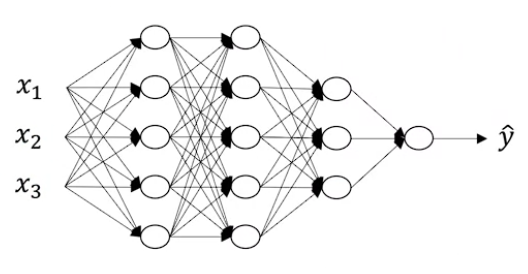
\includegraphics[width=8cm]{11.png}
        \end{figure}
        \begin{itemize}
            \item Above network has 4 layers, $L=4$
            \item $n^{[l]}=$ number of units in layer $l$
            \item $a^{[l]}=$ activations in layer $l$
        \end{itemize}
        \item The inputs $x$ are the activations of the first layer, $x=a^{[0]}$
        \begin{itemize}
            \item Prediction $\hat{y}$ will be the activations of the last layer, $\hat{y}=a^{[L]}$
        \end{itemize}
        \item Forward propagation for a deep NN will follow the same pattern for all layers
        $$z^{[l]}=w^{[l]}a^{[l-1]}+b^{[l]}$$
        $$a^{[l]}=g^{[l]}(z^{[l]})$$
        \item For a vectorized implementation
        $$Z^{[l]}=W^{[l]}A^{[l-1]}+b^{[l]}$$
        $$A^{[l]}=g^{[l]}(z^{[l]})$$
        \begin{itemize}
            \item Explicit for loop will be used to loop over the layers in the network
            \item $b$ will still be a column vector but will apply correctly due to broadcasting
            \item When working with $W$ and $A$ matrices, $A$ will be for the previous layer so the dimensions will fit
        \end{itemize}
        \item When debugging NN, can look at dimensions of all the matrices
        \item For a non vectorized implementation:
        \begin{itemize}
            \item $W^{[l]}:(n^{[l]},n^{[l-1]})$
            \item $b^{[l]}:(n^{[l]},1)$
            \item Dimensions of $dw$ and $db$ should be the same as the dimensions of $W$ and $b$
            \item $a^{[l]}, z^{[l]}:(n^{[l]},1)$ 
        \end{itemize}
        \item For a vectorized implementation, $z$ vectors and $a$ vectors will be stacked horizontally for all training examples
        \begin{itemize}
            \item $Z^{[l]},A^{[l]}:(n^{[l]},m)$
        \end{itemize}
        \item Deep NN tend to work better as each layer can compute increasingly complex functions
        \begin{itemize}
            \item Face recognition: edge detection $\rightarrow$ individual features $\rightarrow$ large parts of the face
            \item Audio: low level waveforms $\rightarrow$ phonemes $\rightarrow$ words $\rightarrow$ sentences
        \end{itemize}
        \item Functions that can be computed with a ``small'' deep neural network require exponentially more hidden units in a shallower network
        \item For each forward propagation step, the value of $z^{[l]}$ should be cached for backpropagation
        \begin{itemize}
            \item Values of $w^{[l]}$ and $b^{[l]}$ can also be stored in the cache so they can be accessed for backpropagation
        \end{itemize}
        \begin{figure}[ht]
            \centering
            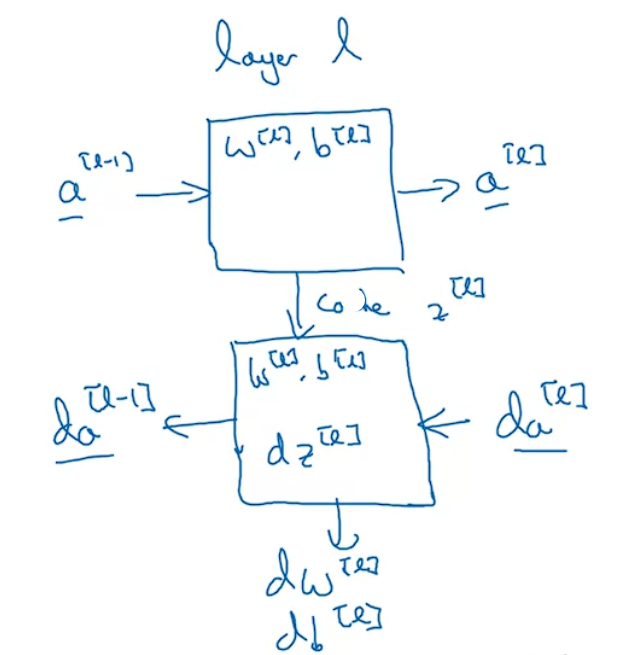
\includegraphics[width=8cm]{12.png}
        \end{figure}
        \item All forward propagation steps will carried out until the hypothesis, $\hat{y}$ is found
        \begin{itemize}
            \item Using cached values, all backpropagation steps will be carried out until $dz^{[1]}$
            \item Parameters $W^{[l]}$ and $b^{[l]}$ can be updated accordingly
            $$W^{[l]}:=W^{[l]}-\alpha dw^{[l]}$$
            $$b^{[l]}:=b^{[l]}-\alpha db^{[l]}$$
        \end{itemize}
        \item Backpropagation will also follow a pattern for all layers in the NN
        \begin{itemize}
            \item $dz^{[l]}=da^{[l]}*g^{[l]'}(z^{[l]})$
            \item $dW^{[l]}=dz^{[l]}a^{[l-1]T}$
            \item $db^{[l]}=dz^{[l]}$
            \item $da^{[l-1]}=W^{[l]T}dz^{[l]}$
        \end{itemize}
        \item For a vectorized implementation:
        \begin{itemize}
            \item $dZ^{[l]}=dA^{[l]}*g^{[l]'}(Z^{[l]})$
            \item $dW^{[l]}=\frac{1}{m}dZ^{[l]}A^{[l-1]T}$
            \item $db^{[l]}=\frac{1}{m}\texttt{np.sum}(dZ^{[l]}\texttt{, axis=1, keepdims=True})$
            \item $dA^{[l-1]}=W^{[l]T}dZ^{[l]}$
        \end{itemize}
    \end{itemize}
    \subsubsection{Parameters vs Hyperparameters}
    \begin{itemize}
        \item Parameters of the NN are the $W$ and $b$ matrices
        \item NN also has a number of associated hyperparameters:
        \begin{itemize}
            \item Learning rate $\alpha$
            \item Number of iterations z`'
            \item Number of layers in the network
            \item Number of hidden units
            \item Choice of activation function
        \end{itemize}
        \item Hyperparameters will control the values of $W$ and $b$
        \item Deep learning has many more hyperparameters than earlier eras of machine learning
        \begin{itemize}
            \item Applying deep learning becomes an empirical process
        \end{itemize}
        \item Intuitions about hyperparameters may be different across different applications
    \end{itemize}
    \pagebreak

    \section{Improving Deep Neural Networks: Hyperparameter Tuning, Regularization and Optimization}
    \subsection{Practical Aspects of Deep Learning}
    \begin{itemize}
        \item Applying ML is a highly iterative process
        \begin{itemize}
            \item Very hard to choose ``correct'' values for hyperparameters
        \end{itemize}
        \begin{figure}[ht]
            \centering
            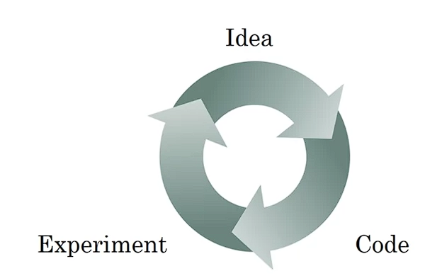
\includegraphics[width=8cm]{13.png}
        \end{figure}
        \item Deep learning used in many different areas
        \begin{itemize}
            \item NLP
            \item Computer vision 
            \item Speech analysis
            \item Structured data
            \begin{itemize}
                \item Advertisement
                \item Search engines
                \item Computer security
                \item Logistics 
            \end{itemize}
        \end{itemize}
        \item Intuitions from one subject area often don't transfer to another application
        \item Success of deep learning can depend on speed of iteration
        \begin{itemize}
            \item Choice of split of the data can influence speed of iteration
        \end{itemize}
        \item Whole dataset should be split into training, development and test set
        \begin{itemize}
            \item Dev set should be used rate performance of different models
            \item Final model should be evaluated on the test set
            \item Split will allow better evaluation of bias and variance of the model
        \end{itemize}
        \item Previous eras of ML had a 60/20/20 split between dataset
        \item For the big data era, a smaller percentage of data is given to the dev and test sets
        \begin{itemize}
            \item For 1,000,000 examples, can allocate just 10,000 examples each to dev and test set
            \item 10,000 examples is enough to run the algorithm and get a good idea about the algorithm performance
        \end{itemize}
        \item Recent trends also show mismatched training and test set distributions
        \begin{itemize}
            \item For images, training set may have very high quality images while test set may have lower quality
            \item Dev and test set should come from the same distribution
        \end{itemize}
        \item Dataset might be split to not include a test set
        \begin{itemize}
            \item Dev set can be used to get to a ``good'' model
            \item Since data is fit to the dev set, there is no unbiased estimate of performance
            \item When data doesn't include a test set, dev set is usually referred to as ``test'' set 
            \item Resulting model may overfit to the dev set
        \end{itemize}
    \end{itemize}
    \subsubsection{Bias and Variance}
    \begin{itemize}
        \item In the deep learning era, there tends to be less of a discussion about the bias/variance trade off
        \item In 2 dimensions, data can be plotted to look for high bias or variance
        \begin{itemize}
            \item High bias classifiers underfit the data
            \item High variance classifiers overfit the data
        \end{itemize}
        \item For higher dimensions, training set error and dev set error can be used
        \begin{itemize}
            \item High variance classifier has low training error and high dev set error
            \item High bias classifier has high training error and high dev set error
            \item Classifier with high bias and high variance will have high training error and even higher dev set error
        \end{itemize}
        \item Above ideas only work with the assumption that the optimal error is 0\%
        \begin{itemize}
            \item Training and dev set must also come from the same distribution
        \end{itemize}
    \end{itemize}
    \subsubsection{Basic Recipe for Machine Learning}
    \begin{itemize}
        \item Train initial algorithm and reduce bias of algorithm to an ``acceptable value''
        \begin{itemize}
            \item Use a larger network 
            \item Train algorithm for longer
        \end{itemize}
        \item Reduce variance of the algorithm by getting more data
        \begin{itemize}
            \item Add regularization terms to the cost function
        \end{itemize}
        \item Bias and variance can also be reduced by using a more appropriate NN architecture
        \item In the big data era, bias and variance can be reduced without affecting each other
        \begin{itemize}
            \item Training a bigger network typically reduce the bias 
            \item Getting more training data will typically reduce the variance
        \end{itemize}
        \item Using regularization will have a bias variance trade off
    \end{itemize}
    \subsubsection{Regularization}
    \begin{itemize}
        \item Adding regularization will usually help in reducing variance and prevent overfitting
        \begin{itemize}
            \item Regularization will only affect how the weights change during backpropagation
            \item For forward propagation, regularization has no effect
        \end{itemize}
        \item For logistic regression:
        $$J(w,b)=\frac{1}{m}\sum_{i=1}^m\mathcal{L}(\hat{y}^{(i)}, y^{(i)})+\frac{\lambda}{2m}||w||_2^2$$
        \begin{align*}
            ||w||_2^2&=\sum_{j=1}^{n_x}w_j^2 \\
            &=w^Tw
        \end{align*}
        \begin{itemize}
            \item Above method is $L_2$ regularization after the $L_2$ norm (Euclidean norm) of $w$
            \item $b$ values can also be regularized but will have a much smaller effect than $w$ 
        \end{itemize}
        \item $L_1$ regularization adds the term:
        $$\frac{\lambda}{m}\sum_{i=1}^{n_x}|w|=\frac{\lambda}{m}||w||_1$$
        \begin{itemize}
            \item Using $L_1$ regularization will result in $w$ being sparse
            \item Can be seen to compressing the model
        \end{itemize}
        \item $L_2$ regularization is more common for deep learning 
        \item Regularization parameter $\lambda$ will be set using the cross validation set
        \begin{itemize}
            \item \texttt{lambda} is a reserved keyword in Python 
        \end{itemize}
        \item For a neural network:
        $$J(w^{[1]},b^{[1]},...,w^{[l]}, b^{[l]})=\frac{1}{m}\sum_{i=1}^m\mathcal{L}(\hat{y}^{(i)}, y^{(i)})+\frac{\lambda}{2m}\sum_{l=1}^L||w^{[l]}||^2$$
        $$||w^{[L]}||^2=\sum^{n^{[l]}}_{i=1}\sum_{j=1}^{n^{[l-1]}} (w^{[l]}_{i,j})^2$$
        \begin{itemize}
            \item $||W^{[l]}||^2_F$ known as the Frobenius norm of the matrix
        \end{itemize}
        \item Since new term added to cost function, $\frac{\partial J}{\partial W^{[l]}}$ will be different
        $$dW^{[l]}=...+\frac{\lambda}{m}W^{[l]}$$
        $$W^{[l]}=W^{[l]}-\frac{\alpha\lambda}{m}W^{[l]}-\alpha(...)$$ 
        \begin{itemize}
            \item Also known as weight decay as value of $W$ will decrease on every iteration
            $$W^{[l]}-\frac{\alpha\lambda}{m}W^{[l]}=\left(1-\frac{\alpha\lambda}{m}\right)W^{[l]}$$
            \item Value of $\left(1-\frac{\alpha\lambda}{m}\right)$ will be slightly less than 1
        \end{itemize}
        \item Adding regularization term will penalize the weight matrix from being too large
        \begin{itemize}
            \item As the value of $\lambda$ is increased, the weights in $w$ will get closer to 0 
            \item Each hidden unit will have a smaller effect and the resulting NN will be simpler
        \end{itemize}
        \item When using the tanh function, penalizing $w$ will make $z^{[l]}$ smaller
        \begin{itemize}
            \item For a small $z^{[l]}$, tanh function is roughly linear
            \item If all hidden units in the network are roughly linear, the result of the NN will also be roughly linear
        \end{itemize}
    \end{itemize}

    \vspace{5mm}
    \textbf{Dropout Regularization}
    \begin{itemize}
        \item Each layer in the NN has a probability of eliminating a node
        \begin{itemize}
            \item When a node is eliminated, all outgoing links from the node are also deleted
            \item Each example will be trained on a smaller network so will have less chance of overfitting 
        \end{itemize}
        \item For each different training example, the NN is reset and randomly eliminates nodes again
        \item Inverted dropout:
        \begin{minted}{Python}
    d3 = np.random.rand(a3.shape[0], a3.shape[1]) < keep_prob
    a3 = np.multiply(a3, d3)
    a3 /= keep_prob
        \end{minted}
        \begin{itemize}
            \item For \texttt{keep\_prob} = 0.8  each node has a 0.2 chance of being removed
            \item Activation values should be scaled by \texttt{keep\_prob} so the expected value of $z$ can stay constant
            \item On each pass through the training set, a different set of units should be zeroed out   
        \end{itemize}
        \item At test time, dropout should not be used as it will create noise in the predictions
        \item A single hidden unit cannot rely on a specific feature as it may not be used on each iteration
        \begin{itemize}
            \item Weights for the unit will be spread out between the units
            \item Has the same effect as shrinking the weights like L2 regularization
            \item The equivalent L2 penalty on different weights depends on the size of the activations being used for the weight
        \end{itemize}
        \item \texttt{keep\_prob} can be varied between the layers
        \begin{itemize}
            \item Larger layers may be more prone to overfitting and can have a larger \texttt{keep\_prob}
            \item For small layers with a very small chance of overfitting, \texttt{keep\_prob} can be set to 1
        \end{itemize}
        \item Many dropout implementations started with computer vision
        \begin{itemize}
            \item Input size for computer vision is extremely large
        \end{itemize}
        \item Cost function is not well defined when dropout is used
        \begin{itemize}
            \item Can set \texttt{keep\_prob} to 1 and check for monotonically decreasing $J$
            \item When $J$ is decreasing, then can reduce the value of \texttt{keep\_prob} to use dropout
        \end{itemize}
    \end{itemize}
    
    \vspace{5mm}
    \textbf{Other Regularization Methods}
    \begin{itemize}
        \item Getting more training data will almost always help overfitting
        \begin{itemize}
            \item May not be possible to get more training data or very expensive
        \end{itemize}
        \item Data augmentation will create new examples and can help reduce overfitting
        \item For an image dataset:
        \begin{itemize}
            \item Flipping the image horizontally
            \item Randomly cropping and distorting the image
        \end{itemize}
        \item Magnitude of image transformation depends on classifier
        \begin{itemize}
            \item For a cat dataset, image should not be flipped vertically 
            \item For OCR, distortions and rotations can be slightly more extreme
        \end{itemize}
        \vspace{5mm}
        \begin{figure}[ht]
            \centering
            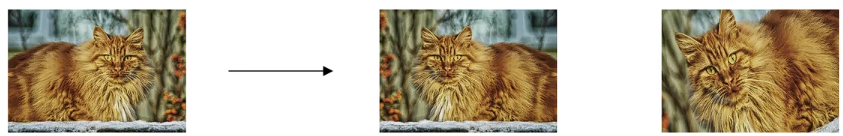
\includegraphics[width=12cm]{14.png}
            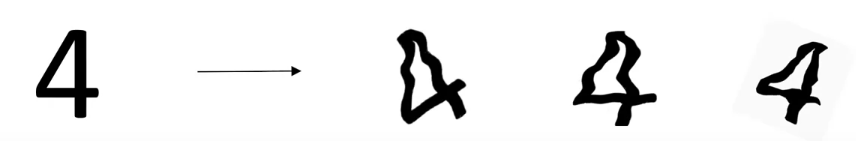
\includegraphics[width=12cm]{15.png}
        \end{figure}
        \item Early stopping can be used to prevent overfitting from happening
        \begin{itemize}
            \item If the NN is overfitting the data, the dev set error will initially decrease before increasing
            \item Training of the NN can be stopped when the dev set error is lowest and the data has not been overfit
        \end{itemize}
        \item Using early stopping links the task of optimizing $J$ and not overfitting the data
        \begin{itemize}
            \item Early stopping will prevent the cost function from being optimized 
        \end{itemize}
        \item L2 regularization is a better method to prevent overfitting
        \begin{itemize}
            \item Requires a choice for the value of $\lambda$ and is much more computationally expensive
        \end{itemize}
    \end{itemize}
    \subsubsection{Setting up the Optimization Problem}
    \begin{itemize}
        \item Normalization can be used to speed up the training of a NN
        \begin{itemize}
            \item Subtract the mean:
            $$\mu=\frac{1}{m}\sum_{i=1}^mx^{(i)}$$
            $$x:=x=\mu$$
            \item Normalize the variance:
            $$\sigma^2=\frac{1}{m}\sum_{i=1}^mx^{(i)}**2$$ 
            $$x/=\sigma$$
        \end{itemize}
        \item When normalizing a training set, test set and training set should be processed together
        \begin{itemize}
            \item All the data must go through the same transformation
        \end{itemize}
        \item For data that is not normalized, the cost function will be very elongated
        \begin{itemize}
            \item The gradient will be quite shallow and will take longer to converge
            \item Algorithm will require a smaller learning rate
            \vspace{5mm}
            \begin{figure}[ht]
                \centering
                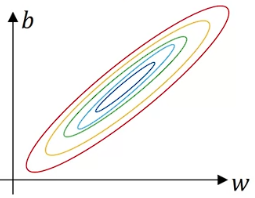
\includegraphics[width=8cm]{18.png}
            \end{figure}
        \end{itemize}
        \item On average, normalized data will have a cost function that is more symmetric
        \begin{itemize}
            \item Gradient descent will converge faster and can use a larger learning rate
            \begin{figure}[ht]
                \centering
                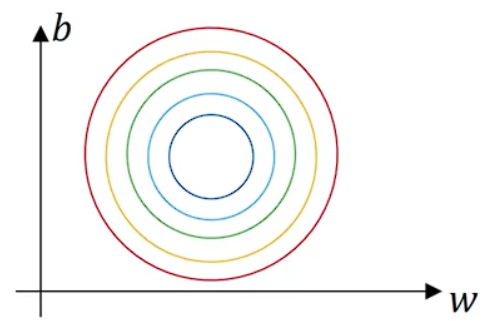
\includegraphics[width=8cm]{19.png}
            \end{figure}
        \end{itemize}
    \end{itemize}

    \vspace{5mm}
    \textbf{Vanishing/Exploding Gradients}
    \begin{itemize}
        \item For very deep neural networks, the derivatives can get exponentially big or small
        \item If the weights of a NN are all the same, the prediction $\hat{y}$ will $x$ to the $L$th power
        \begin{itemize}
            \item For $W^{[l]}>I$ the gradient will explode
            \item For $W^{[l]}<I$ the gradient will vanish
        \end{itemize}
        \item Some modern applications use 152 layer NN
        \begin{itemize}
            \item Require careful initialization of the weights to ensure correct training
        \end{itemize}
        \item For a single neuron:
        \begin{itemize}
            \item The output $\hat{y}$ will be the sum of all $w_ix_i$
            $$z = w_1x_1+w_2x_2+...+w_nx_n$$
            \item For a large $n$, want a smaller $w_i$
            \item Want $\text{Var}(w_i)=\frac{1}{n}$
        \end{itemize}
        \begin{minted}[escapeinside=||]{Python}
    |$W^{[l]}$| = np.random.randn(shape) * np.sqrt|$\left(\frac{1}{n^{[l-1]}}\right)$|
        \end{minted}
        \begin{itemize}
            \item Variance of Gaussian random variable can be set by multiplying by sqrt tem
        \end{itemize}
        \item For ReLU activation function, the variance should be set to $\frac{2}{n}$
        \begin{itemize}
            \item tanh activation uses Xavier initialization $\frac{1}{n^{[l-1]}}$
            \item Yoshua Bengio multiplied random variable by $\sqrt{\frac{2}{n^{[l-1]}+n^{[l]}}}$
        \end{itemize}
        \item Initialization of weights aims to set weight matrices close to 1
        \begin{itemize}
            \item Helps to prevent $\hat{y}$ from vanishing or exploding too quickly
        \end{itemize}
        \item Variance parameter can be tuned as another hyperparameter
    \end{itemize}

    \vspace{5mm}
    \textbf{Gradient Checking}
    \begin{itemize}
        \item Can be used to ensure implementation of backpropagation is correct
        \item Requires numerical approximations of gradients
        \begin{itemize}
            \item For a function $f$ at a point $\theta$, gradient can be approximated by looking at $\theta+\epsilon$ and $\theta-\epsilon$
            \item Approximation is closer when double sided estimate is used
        \end{itemize}
        \item If $g$ is the derivative of $f$:
        $$g(\theta)\approx\frac{f(\theta+\epsilon)-f(\theta-\epsilon)}{2\epsilon}$$
        \item Using the 2 sided difference will give a much better estimate but is more computationally expensive
        \item The derivative of a function at a point is the limit of the numerical approximation
        $$f'(\theta)=\lim_{\epsilon\rightarrow 0}\frac{f(\theta+\epsilon)-f(\theta-\epsilon)}{2\epsilon}$$
        \begin{itemize}
            \item For a non 0 value of $\epsilon$, the error of the approximation is $O(\epsilon^2)$
            \item For the single sided numerical approximation, the error is $O(\epsilon)$ 
        \end{itemize}
        \item To perform gradient checking on a NN:
        \begin{enumerate}
            \item Reshape $W^{[1]},b^{[1]},...,W^{[L]},b^{[L]}$ into a single vector $\theta$
            \item Reshape $dW^{[1]},db^{[1]},...,W^{[L]},b^{[L]}$ into a single vector $d\theta$
            \item For every $i$ in $\theta$, calculate:
            $$d\theta_{approx}[i]=\frac{J(\theta_1,\theta_2,...,\theta_i+\epsilon)-J(\theta_1,\theta_2,...,\theta_i-\epsilon)}{2\epsilon}$$
            \item Check if $d\theta_{approx}$ and $d\theta$ are reasonably close to each other
            
            For $\epsilon=10^{-7}$:
            $$\frac{||d\theta_{approx}-d\theta||_2}{||d\theta_{approx}||_2+||d\theta||_2}\approx 10^{-7}$$
        \end{enumerate}
        \item Grad check should be only be used when debugging
        \begin{itemize}
            \item Calculating $d\theta_{approx}$ is very computationally expensive
        \end{itemize}
        \item If regularization is used, correct cost function must be used to calculate the gradient
        \item If dropout is used, $J$ is not well defined and cannot use grad check
        \begin{itemize}
            \item Cost function $J$ that is optimized by dropout is defined by summing over all subsets of nodes that could be eliminated on each iteration
            \item Can implement grad check with a \texttt{keep\_prob} of 1 before turning on dropout
        \end{itemize}
        \item Implementation of gradient descent may be correct when $W$ and $b$ are close to 0
        \begin{itemize}
            \item Can run grad check just after random initialization
            \item After training the network for a number of iterations, can run grad check again
        \end{itemize}
    \end{itemize}

    \subsection{Optimization Algorithms}
    \subsubsection{Mini Batch Gradient Descent}
    \begin{itemize}
        \item For gradient descent, vectorization will allow computation over all $m$ training examples
        \begin{itemize}
            \item If $m$ is very large, then vectorization will still be very slow
        \end{itemize}
        \item Gradient descent requires the whole training set to be processed for a single step of gradient descent
        \item Data from training set can be split into mini batches
        $$X^{\{1\}}=[x^{(1)},x^{(2)},...,x^{(1000)}]$$
        $$Y^{\{1\}}=[y^{(1)},y^{(2)},...,y^{(1000)}]$$
        \item Mini batch gradient descent looks at one mini batch on each iteration of gradient descent
        \item For each mini batch in the training set:
        \begin{itemize}
            \item Run forward propagation on $X^{\{t\}}$
            \begin{itemize}
                \item[] $Z^{[1]}=W^{[1]}X^{\{t\}}+b^{[1]}$
                \item[] $A^{[1]}=g^{[1]}(Z^{[1]})$
                \item[] ...
                \item[] $A^{[l]}=g^{[l]}(Z^{[l]})$
            \end{itemize}
            \item Compute cost: $J^{\{t\}}=\frac{1}{1000}\sum_{i=1}^l\mathcal{L}(\hat{y}^{(i)},y^{(i)})+\frac{\lambda}{2\times 1000}\sum_l||W^{[l]}||_F^2$
            \item Use backpropagation to calculate gradients wrt $J^{\{t\}}$
            \item Update weights
            \begin{itemize}
                \item[] $W^{[l]}:=W^{[l]}-\alpha dW^{[l]}$
                \item[] $b^{[l]}:=b^{[l]}-\alpha db^{[l]}$
            \end{itemize}
        \end{itemize}
        \item A single pass through the training set is known as an epoch
        \item Algorithm can continue to run for multiple passes through the training set until an optimal solution is found
        \item For batch gradient descent, the cost should decrease on each iteration
        \begin{itemize}
            \item If the cost doesn't decrease per iteration, then the algorithm has a bug
        \end{itemize}
        \item For mini batch gradient descent, the cost will trend downwards but will be more noisy
        \begin{itemize}
            \item Algorithm is being trained on a different batch of results on each iteration
        \end{itemize}
        \item When running mini batch gradient descent, must choose the size of the mini batch
        \begin{itemize}
            \item For mini batch size = $m$: Batch gradient descent
            \item For mini batch size = 1: Stochastic gradient descent
        \end{itemize}
        \item For stochastic gradient descent, each example may be good or bad for gradient descent
        \begin{itemize}
            \item On average the cost function will be minimized for gradient descent
            \item Path taken by gradient descent will be very noisy
            \item Stochastic gradient descent will never converge and just oscillate around the minimum
        \end{itemize}
        \item Choice of mini batch size should be between 1 and $m$
        \begin{itemize}
            \item Batch gradient descent will take very long for a single iteration
            \item Stochastic gradient descent will lose all the speed from vectorization
        \end{itemize}
        \item For a small training set ($m\leq 2000$), can just use gradient descent
        \item Otherwise can try a mini batch size from 64-512
        \begin{itemize}
            \item Code may run faster if the mini batch size is a power of 2
        \end{itemize}
        \item A single mini batch should be able to fit in the whole CPU/GPU memory
    \end{itemize}

    \vspace{5mm}
    \textbf{Advanced Optimization Algorithms}
    \begin{itemize}
        \item Some advanced algorithms require the use of exponentially weighted averages
        \item Moving averages can be calculated for data such as daily temperature
        $$V_0=0$$
        $$V_t=\beta V_{t-1}+(1-\beta)\theta_t$$
        \begin{itemize}
            \item $V_t$ is the approximated average temperature over the last $\frac{1}{1-\beta}$ days 
            \item If $\beta$ is larger then the average will adapt slower to changes in the data
        \end{itemize}
        \item Exponentially weighted average can be found by summing the daily temperature with an exponentially decaying function 
        \item If $\beta=0.9$:
        $$V_{100}=0.1\theta_{100}+(0.1)(0.9)\theta_{99}+(0.1)(0.9)^2\theta_{98}+(0.1)(0.9)^3\theta_{97}+...$$ 
        \item When calculating the exponentially weighted average, the same variable $v$ should be used and overwritten each time
        \begin{itemize}
            \item Implementation will be much more efficient than calculating average manually from the past 10 values 
        \end{itemize}
        \item For large values of $\beta$, initial average will be much lower than they should be 
        $$\frac{V_t}{1-\beta^t}$$
        \item Bias correction can be used to ensure initial values are correct estimations of the averages
        \begin{itemize}
            \item As $t$ becomes larger, denominator becomes closer to 1
        \end{itemize}
    \end{itemize}

    \vspace{5mm}
    \textbf{\textit{Momentum}}
    \begin{itemize}
        \item Gradient descent with momentum uses an exponentially weighted average of the gradients to update the weights
        \begin{itemize}
            \item Almost always performs better than standard gradient descent
            \item[] $V_{dW}=\beta V_{dW}+(1-\beta)dW$
            \item[] $V_{db}=\beta V_{db}+(1-\beta)db$
            \item[] $W=W-\alpha V_{dw}$
            \item[] $b=b-\alpha V_{db}$
        \end{itemize}
        
        
        
        \item Taking the average of the gradients will slow down any unnecessary oscillations in the algorithm
        \begin{itemize}
            \item Algorithm may oscillate at first but will start to take more direct steps to the minimum
        \end{itemize}
        \item $\beta=0.9$ is a common choice for most applications of momentum
    \end{itemize}

    \vspace{5mm}
    \textbf{\textit{RMSprop}}
    \begin{itemize}
        \item RMSprop takes the weighted average of the squares of the derivatives
        \item Derivatives will get divided by the RMS before the weights are updated
        \begin{itemize}
            \item[] $S_{dW}=\beta_2S_{dW}+(1-\beta)dW^2$
            \item[] $S_{db}=\beta_2S_{db}+(1-\beta)db^2$
            \item[] $W=W-\alpha\frac{dW}{\sqrt{S_{dw}}}$
            \item[] $b=b-\alpha\frac{db}{\sqrt{S_{db}}}$
        \end{itemize}
        \item Updates in the direction of oscillation will be divided by a large number
        \begin{itemize}
            \item Will allow the learning rate to be larger and therefore allows faster training
        \end{itemize}
        \item In practice, very small value $\epsilon$ is added to the denominator for more numerical stability
    \end{itemize}

    \vspace{5mm}
    \textbf{\textit{Adam Optimization Algorithm}}
    \begin{itemize}
        \item Adam optimization shown to work well for a range of deep learning architectures
        \begin{itemize}
            \item Merges Momentum and RMSprop to one algorithm 
            \item ``Adam'' stands for adaptive moment estimation
        \end{itemize}
        \item On iteration $t$:
        \begin{itemize}
            \item[] Compute $dW,db$ using the current mini batch
            \item[] $V_{dw}=\beta_1V_{dw}+(1-\beta_1)dW,~~V_{db}=\beta_1V_{db}+(1-\beta_1)db$
            \item[] $S_{dw}=\beta_2S_{dw}+(1-\beta_2)dW^2,~~S_{db}=\beta_2s{db}+(1-\beta_2)db^2$
            \item[] $V_{dw}^{C}=\frac{V_{dw}}{1-\beta_1^t},~~V_{db}^{C}=\frac{V_{db}}{1-\beta_1^t}$
            \item[] $S_{dw}^{C}=\frac{S_{dw}}{1-\beta_2 ^t},~~S_{db}^{C}=\frac{S_{db}}{1-\beta_2 ^t}$
            \item[] $W:=W-\alpha\frac{V_{dw}^{C}}{\sqrt{S_{dw}^{C}}+\epsilon}$
            \item[] $b:=b-\alpha\frac{V_{db}^C}{\sqrt{S_{db}^C}+\epsilon}$
        \end{itemize}
        \item Must choose many hyperparameters to run Adam optimization
        \begin{itemize}
            \item $\alpha$: needs to be tuned to the specific NN
            \item $\beta_1$: 0.9 (default)
            \item $\beta_2$: 0.999 (default)
            \item $\epsilon: 10^{-8}$ (default) 
        \end{itemize}
    \end{itemize}

    \vspace{5mm}
    \textbf{Learning Rate Decay}
    \begin{itemize}
        \item For mini batch gradient descent, the algorithm will oscillate around the minimum point
        \item If the learning rate is reduced over time, then the oscillations will become smaller 
        \begin{itemize}
            \item During the initial steps of learning, algorithm can afford to take large steps
            \item As the algorithm starts to converge, smaller steps are preferred
        \end{itemize}
        $$\alpha=\frac{1}{1+\text{decay rate $\times$ epoch num}}\alpha_0$$
        \item Other formulas can be used to decay the learning rate
        \begin{itemize}
            \item Exponential decay
            $$\alpha=0.95^{\text{epoch num}}\alpha_0$$
            \item Discrete staircase
            \begin{figure}[ht]
                \centering
                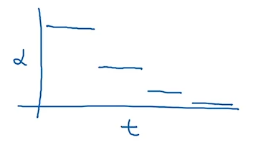
\includegraphics[width=8cm]{20.png}
            \end{figure}
            \item Square root of epoch number
            $$\alpha=\frac{k}{\sqrt{\text{epoch num}}}\alpha_0$$            
        \end{itemize}
        \item Manual decay can be used for larger models that take a longer time to train
    \end{itemize}

    \vspace{5mm}
    \textbf{Local Optima}
    \begin{itemize}
        \item Initial ideas believed that a cost function with many points of 0 gradient would have many local optima
        \begin{itemize}
            \item When training a NN, most points with 0 gradient are saddle points
        \end{itemize}
        \begin{figure}[ht]
            \centering
            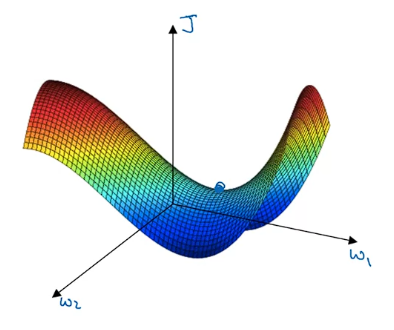
\includegraphics[width=8cm]{21.png}
        \end{figure}
        \item For a point with 0 gradient, Each direction can either be a convex or concave function
        \begin{itemize}
            \item For a local optima, must have a convex function in all directions
            \item In a high dimensional space, chance of all directions being convex functions is very small
        \end{itemize}
        \item Intuitions about lower dimensional spaces may not transfer to high dimensional spaces
        \item Plateaus are areas where the gradient is near to 0 for a large area
        \begin{figure}[ht]
            \centering 
            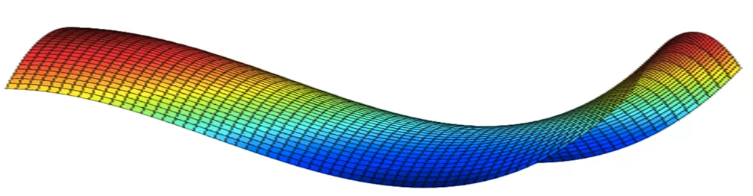
\includegraphics[width=12cm]{22.png}
        \end{figure}
        \begin{itemize}
            \item Will take a very long time to move down off the plateau
            \item Learning will be slow but unlikely to get stuck in a local optima
        \end{itemize}
        \item Optimization algorithms like Adam can help to speed up the training
    \end{itemize}

    \subsection{Hyperparameter Tuning, Batch Normalization and Programming Frameworks}
    \subsubsection{Hyperparameter Tuning}
    \begin{itemize}
        \item Deep neural networks have many hyperparameters associated with the actual network and the training implementation
        \begin{itemize}
            \item Numbers of layers and hidden units
            \item Learning rate or method for learning rate decay
            \item Hyperparameters for momentum or Adam optimization
            \item Mini batch size 
        \end{itemize}
        \item Most important hyperparameter is the learning rate
        \begin{itemize}
            \item Secondary importance can be given to momentum ($\beta$), number of hidden units and the mini batch size
            \item Number of layers and learning rate decay can be tuned last
            \item Parameters for Adam optimization usually don't need to be tuned
        \end{itemize}
        \item In practice, random values for the hyperparameters should be sampled and tested
        \begin{itemize}
            \item If values are arranged in a grid, fewer distinct values can be tested
            \item Choosing random values for the hyperparameters gives a higher chance of finding an optimum value for important hyperparameters
        \end{itemize}
        \item Can use coarse to fine sampling scheme to find optimum values
        \begin{itemize}
            \item Sample initial values and find which values work the best
            \item ``Zoom in'' to the area and take more samples in the smaller region
        \end{itemize}
        \item For some hyperparameters (number of layers / hidden units), can sample over a reasonable range 
        \item Some hyperparameters may not have an even distribution (Learning rate between 0.0001 and 1)
        \begin{itemize}
            \item Can use a log scale to ensure the numbers are better distributed 
            \begin{minted}{Python}
    r = -4 * np.random.rand
    learning_rate = 10 ** r
            \end{minted}
            \item Can look for a range $10^a ... 10^b$ and take a random sample $r\in[a,b]$
        \end{itemize}
        \item For exponentially weighted averages, $\beta$ will be around 0.9-0.999
        \begin{itemize}
            \item Equivalent to averaging over the last 10 days or last 1000 days
            \item Can sample values for $1-\beta$ for $r\in[-3,-1]$
        \end{itemize}
        \item For exponentially weighted averages, the sensitivity of the results is very high when $\beta$ is close to 1
        \begin{itemize}
            \item A change from 0.999 to 0.9995 will change the average from 1000 to 2000 examples
        \end{itemize}  
        \item Intuitions about the hyperparameters won't always transfer across applications
        \begin{itemize}
            \item Ideas found in one application can still be applied to other applications
        \end{itemize} 
        \item Hyperparameters can become stale over time with changing data or hardware
        \begin{itemize}
            \item Hyperparameters should be reevaluated every few months to ensure values are optimal
        \end{itemize}
        \item Depending on resources, can babysit a single model or train models in parallel 
        \begin{itemize}
            \item For a single model, hyperparameters can be tweaked over time depending on training performance
            \item If resources allow, can train the same model with many different hyperparameters and choose the best model
        \end{itemize}
    \end{itemize}

    \subsubsection{Batch Normalization}
    \begin{itemize}
        \item Inputs to a NN can be normalized to speed up learning
        $$X=\frac{X-\mu}{\sigma}$$
        \item Batch normalization normalizes the input values $Z^{[l]}$ to each layer
        \begin{itemize}
            \item Can instead normalize the values $A^{[l]}$ after the activation function 
        \end{itemize}
        \item Given intermediate values $z^{(1)},...,z^{(m)}$:
        \begin{itemize}
            \item[] $\mu=\frac{1}{m}\sum_iz^{(i)}$
            \item[] $\sigma^2=\frac{1}{m}\sum_i(z^{(i)}-\mu)^2$
            \item[] $z^{(i)}_{norm}=\frac{z^{(i)}-\mu}{\sqrt{\sigma^2+\epsilon}}$
            \item[] $\tilde{z}^{(i)}=\gamma~z_{norm}^{(i)}+\beta$
        \end{itemize}
        \item $\gamma$ and $\beta$ are learnable parameters of the model
        \begin{itemize}
            \item Allows the mean and variance of $\tilde{z}$ to be set to any value
            \item If $\gamma=\sqrt{\sigma^2+\epsilon}$, $\beta=\mu$, then $\tilde{z}^{(i)}=z^{(i)}$
            \item May not want mean 0 and standard deviation 1 for the activation function
        \end{itemize}
        \item NN will have new parameters $\beta^{[1]},\gamma^{[1]},...,\beta^{[L]},\gamma^{[L]}$
        \begin{itemize}
            \item Will be updated like normal parameters
            $$\beta^{[l]}=\beta^{[l]}-\alpha d\beta^{[l]}$$
            $$\gamma^{[l]}=\gamma^{[l]}-\alpha d\gamma^{[l]}$$
        \end{itemize}
        \item Batch normalization is typically applied to mini batch gradient descent
        \begin{itemize}
            \item Mean and variance will be calculated from the mini batch being used 
        \end{itemize}
        \item When using batch normalization, normalization step removes the need for $b^{[l]}$ parameters
        \begin{itemize}
            \item When subtracting the mean from the $z$ values, the constant will get cancelled out
            \item Mean of the $\tilde{Z}$ values will be decided by the $\beta^{[l]}$ parameters 
        \end{itemize}
        \item Batch normalization will make weights deeper in a network more robust to changes earlier in the network
        \begin{itemize}
            \item Data can have a covariate shift where the distribution changes after a generalization 
            \item Function mapping from $X$ to $Y$ can be the same but model may need to be retrained 
            \item Batch normalization will reduce the amount of movement of the distribution of the hidden values
        \end{itemize}
        \item Even if there is a covariate shift in the data, batch norm will make the $z$ values have the same mean and variance
        \begin{itemize}
            \item The individual layers in the network will be more independent of each other 
        \end{itemize}
        \item Batch norm will also add a slight regularization effect
        \begin{itemize}
            \item Each mini batch is scaled by the mean/variance of the specific mini batch
            \item Normalizing with the mean/variance of the individual mini batch will add noise to the activations
            \item Similar to dropout where the algorithm will not rely on any single hidden unit 
            \item Noise added to the $z$ values is very small so dropout can be used as well 
        \end{itemize}
        \item If a larger mini batch size is used, noise is reduced and will have a smaller regularization effect
        \item At test time, data will typically be processed one example at a time 
        \begin{itemize}
            \item Cannot calculated the mean/variance of a single example 
            \item Mean/variance can be estimated using exponentially weighted averages across the mini batches
        \end{itemize}
    \end{itemize}
    \subsubsection{Multi Class Classification}
    \begin{itemize}
        \item Logistic regression can be generalized to apply to multiple classes
        $$C=\text{number of classes}$$
        \item Output layer for the NN will have $C$ units
        \begin{itemize}
            \item Each unit will be the probability of each class
            \item Sum of all numbers in the vector must be 1
        \end{itemize}
        \item Softmax layer used in the output layer to output vector of probabilities
        \begin{itemize}
            \item $Z^{[L]}$ values are calculated as normal: $Z^{[L]}=W^{[L]}a^{[L-1]}+b^{[L]}$
            \item Use the softmax activation function
            \begin{itemize}
                \item[] $t=e^{(Z^{[L]})}$
                \item[] $a^{[L]}=\frac{t}{\sum_{i=1}^Ct _i}$
            \end{itemize}
        \end{itemize}
        \item Softmax activation function has a vector for its input and output
        \begin{itemize}
            \item Other activation functions had a single value for input and output
        \end{itemize}
        \item Largest input to softmax function will result in the largest output
        \begin{itemize}
            \item ``Hard max'' function would return 1 for the largest input and 0 for the other inputs
        \end{itemize}
        \item If $C=2$, softmax reduces to logistic regression
        \item Softmax classifier cannot be trained as a normal NN
        $$\mathcal{L}(\hat{y},y)=-\sum_{j=1}^Cy_j\log\hat{y}_j$$
        \item Loss function will only be active for the ground truth class in the training set
        $$J(W^{[1]}, b^{[1]},...)=\frac{1}{m}\sum_{i=1}^m\mathcal{L}(\hat{y}^{(i)},y^{(i)})$$
        $$dz^{[L]}=\hat{y}-y$$
    \end{itemize}
    \subsubsection{Deep Learning Frameworks}
    \begin{itemize}
        \item For larger NNs, using a framework can save a lot of time 
        \item Can look at the community behind the frameworks and the strengths
        \begin{itemize}
            \item Ease of programming (development and deployment)
            \item Running speed
            \item Truly open (open source with good governance)
            \item Application of NN
        \end{itemize}
    \end{itemize}

    \vspace{5mm}
    \textbf{Tensorflow}
    \begin{itemize}
        \item Assume a simple cost function:
        $$J(w)=w^2+10w+25$$
    \end{itemize}
    \begin{minted}{Python}
        import numpy as np 
        import tensorflow as tf

        w = tf.Variable(0, dtype=tf.float32)
        optimizer = tf.keras.optimizers.Adam(0.1)

        def train_step():
            with tf.GradientTape() as tape():
                cost = w ** 2 - 10 * w + 25
            trainable_variables = [w]
            grads = tape.gradient(cost, trainable_variables)
            optimizer.apply_gradients(zip(grads, trainable_variables))

        for i in range(1000):
            train_step() 
    \end{minted}
    \begin{itemize}
        \item No need to compute backpropagation steps with tensorflow
        \item More complex tensorflow program will have cost as a function of variables
    \end{itemize}
    \begin{minted}{Python}
        w = tf.Variable(0, dtype=tf.float32)
        x = np.array([1.0, -10.0, 25.0], dtype=np.float32)
        optimizer = tf.keras.optmizers.Adam(0.1)


        def training(x, w, optimizer):
            def cost_fn():
                return x[0] * w ** 2 + x[1] * w + x[2]

            for i in range(1000):
                optimizer.minimize(cost_fn, [w])

            return w  
    \end{minted}
    \begin{itemize}
        \item Tensorflow will create a computation graph from the defined cost function
        \begin{itemize}
            \item From the computation graph, tensorflow will compute the backpropagation steps
        \end{itemize} 
    \end{itemize}
    \pagebreak
    
    \section{Structuring Machine Learning Projects}
    \subsection{ML Strategy} 
    \subsubsection{Setting up a ML Project}
    \begin{itemize}
        \item A machine learning project may have many ideas that can improve performance
        \begin{itemize}
            \item Collect more data
            \item Use a more diverse training set
            \item Train the algorithm over a longer period of time
            \item Use a different optimization algorithm (Adam instead of gradient descent)
            \item Use a bigger/smaller network
            \item Add dropout or $L_2$ regularization
            \item Change the network architecture (activation functions or hidden units)
        \end{itemize}
        \item Some methods may not be useful for the specific scenario
        \item ML strategy is changing with deep learning
        \begin{itemize}
            \item Deep learning algorithms have different options when compared with previous generations
        \end{itemize} 
        \item Orthogonalization is where specific functions can be split up into different areas 
        \item For a supervised learning system to perform well, system requires a chain of assumptions
        \begin{itemize}
            \item Performance of algorithm on the training set must pass some threshold ($\approx$ human-level performance)
            \item Algorithm must be fit well to the dev set
            \item Algorithm must be fit well to the test set
            \item Algorithm must perform well in the real world
        \end{itemize}
        \item Each step has specific ``knobs'' to tune to improve performance in the specific area
        \begin{itemize}
            \item Training set: bigger network, Adam optimization
            \item Dev set: regularization, bigger training set
            \item Test set: bigger dev set 
            \item Real world: change dev set or cost function
        \end{itemize}
        \item Early stopping can be used but is less orthogonalized
        \begin{itemize}
            \item Worsens the performance on the training set 
            \item Improves the performance on the dev set
        \end{itemize}
        \item Single number evaluation metric can be used to test effectiveness of a model
        \item F1 score combines precision and recall into a single metric
        \begin{itemize}
            \item Precision is the percentage of positively classified examples that are actually positive
            \item Recall is the percentage of positive examples that are correctly classified
            \item F1 score takes the harmonic mean of precision and recall
        \end{itemize}
        $$F_1=\frac{2}{\frac{1}{P}+\frac{1}{R}}$$
        \item Having a well defined test set and single number evaluation metric will speed up iteration 
        \item Scenario may have more than one type of metric that is relevant
        \begin{itemize}
            \item Classification algorithm may value accuracy as well as running time
            \item May not make sense to use a numerical function of some metrics
        \end{itemize}
        \item Accuracy would be a optimizing metric and running time would be the satisficing metric
        \begin{itemize}
            \item Goal can be to maximize accuracy subject to running time $\leq$ 100ms
        \end{itemize}
        \item For $N$ different metrics:
        \begin{itemize}
            \item 1 should be optimizing
            \item $N-1$ should be satisficing
        \end{itemize}
        \item Dev set and test set should come from the same distribution
        \begin{itemize}
            \item If different distributions are used, algorithm may perform on the dev set but not on the test set 
            \item Dev set and test set must have the same target
        \end{itemize}
        \item Dev set should be used to evaluate the performance of different models
        \begin{itemize}
            \item Setting up a dev set and an evaluation metric allows teams to iterate quickly
        \end{itemize}
        \vspace{5mm}
        \begin{center}
            ``Choose a dev set and test set to reflect data you expect to get in the future and consider important to do well on''
        \end{center}
        \item Previous eras of machine learning had a 60\%, 20\%, 20\%
        \item Modern eras of machine learning have much larger datasets
        \begin{itemize}
            \item For 1000000 examples, can assign 1\% each to dev and test set
            \item Larger amount of data in the training set will help algorithm 
        \end{itemize}
        \vspace{5mm}
        \begin{center}
            ``Set your test set to be big enough to give high confidence in the overall performance of your system''
        \end{center}
        \item Some applications may only use a train and dev set
        \begin{itemize}
            \item Specific scenario may not require high confidence in the overall performance of the algorithm 
            \item Must be careful to not overfit the dev set too much
        \end{itemize}
        \item Evaluation metric may not give a full representation of the specific scenario
        \begin{itemize}
            \item Cat classifier with very low error may allow some pornographic images through the algorithm
            \item Algorithm with slightly higher error but no pornographic images would be preferred
        \end{itemize}
        \item Evaluation metric should be changed if it doesn't correctly rank the algorithm's performance
        \begin{itemize}
            \item Standard error function treats all images equally 
            \item Weight can be added to the error function to weight unwanted images higher
            \item Requires labelling of unwanted images in dev and test set
        \end{itemize}
        \item Task of changing evaluation metric is separate from changing cost function to achieve good performance
        \item Metric and/or dev/test set should be changed if performance on the application is not linked
    \end{itemize}
    \subsubsection{Comparing to Human Level Performance}
    \begin{itemize}
        \item With advances in deep learning, ML algorithms have much better performance
        \begin{itemize}
            \item More feasible for algorithms to be competitive with human level performers
        \end{itemize}
        \item Workflow of designing and building a ML system is more efficient when trying to learn something that humans can do
        \item For many ML projects, initial learning will be very fast as algorithm approaches human level performance
        \begin{itemize}
            \item Rate of learning decreases after algorithm surpasses human level performance
            \item Algorithm will approach Bayes optimal error
        \end{itemize} 
        \item Bayes optimal error is the best theoretical function for mapping from $X$ to $Y$
        \begin{itemize}
            \item For many tasks, human level performance is not very far from Bayes optimal error
            \item Once human level performance is surpassed, there may not be many areas to improve in
        \end{itemize}
        \item If algorithm has lower than human level performance:
        \begin{itemize}
            \item Get labelled data from humans
            \item Gain insight from manual error analysis 
            \item Better analysis of bias/variance
        \end{itemize}
        \item If human level performance is much lower than the training and dev set error, can focus on the bias of the algorithm  
        \item If human level performance is close to the training error, can focus on the variance of the algorithm
        \item Human level performance can be used as an estimate for Bayes error
        \begin{itemize}
            \item Difference between the Bayes error and training error is the avoidable bias
            \item Difference between the training and dev set error can measure the variance
        \end{itemize}
        \item For specialized tasks, different parties may have different errors for human classification
        \begin{itemize}
            \item For medical image classification, a team of experienced doctors will have much lower error than an average human
            \item Bayes error must be less than or equal to the lowest human error
            \item Lowest human error can be used as estimate for Bayes error 
        \end{itemize}
        \item For publishing a paper or deploying a system, human error definition may be different
        \item When algorithm is very close to human level performance, can be hard to see if bias or variance should be trained
        \item With deep learning, algorithms in some areas can surpass human level performance
        \begin{itemize}
            \item Online advertising
            \item Product recommendations
            \item Logistics
            \item Loan approvals 
        \end{itemize}
        \item Above areas are not natural perception problems and come from structured data
        \begin{itemize}
            \item Currently more challenging for computers to surpass humans in natural perception tasks
        \end{itemize}
        \item ML has also surpassed humans in some natural perception tasks
        \begin{itemize}
            \item Speech recognition
            \item Some image recognition
            \item Medical tasks
        \end{itemize}
        \item For supervised learning, must assume that the training set can be fit well (low avoidable bias)
        \begin{itemize}
            \item The training set performance must also generalize well to the dev/test set (low variance)
        \end{itemize}
        \item For high bias:
        \begin{itemize}
            \item Train a bigger model
            \item Train for longer or use a better optimization algorithm (momentum, RMSprop, Adam)
            \item Change the NN architecture or find better hyperparameters
        \end{itemize}
        \item For high variance:
        \begin{itemize}
            \item Use more data 
            \item Use regularization ($L_2$, dropout, data augmentation)
            \item Change the NN architecture or find better hyperparameters
        \end{itemize}
    \end{itemize} 
    \subsubsection{Error Analysis}
    \begin{itemize}
        \item Misclassified examples can be manually examined to look for any patterns
        \begin{itemize}
            \item Finding patterns can give an upper bound of any increase in performance 
        \end{itemize}
        \item Different ideas for error analysis can be evaluated in parallel with a table
        \begin{itemize}
            \item For each image, can fill in a checkbox for any patterns
            \item Percentage of total for each pattern will give an idea of how to best improve performance
        \end{itemize}
        \item Manual analysis may show new patterns in the errors
        \item Some errors may be incorrectly labelled examples in the dev/test set
        \begin{itemize}
            \item Deep learning algorithms are quite robust to random errors in the training set
            \item Algorithms are fairly susceptible to systematic errors in the training set 
        \end{itemize}
        \item Incorrectly labelled examples can be recorded in the error analysis table
        \begin{itemize}
            \item Percentage of error caused by incorrect labels can be calculated to see if fixing labels is a worthwhile task
        \end{itemize}
        \item Any processes should be applied to the dev and test set at the same time to ensure they come from the same distribution
        \begin{itemize}
            \item Training set may end up coming from a different distribution than the dev/test set
        \end{itemize}
        \item Can also look at examples that the algorithm got right to see if got any errors
        \item For a new ML system, priority should be to build initial system then iterate
        \begin{itemize}
            \item Set up a dev/test set and evaluation metric
            \item Build initial system quickly
            \item Use bias/variance and error analysis to prioritize next steps
        \end{itemize}
        \item Error analysis will give idea for next steps
    \end{itemize}
    \subsubsection{Mismatched Training and Dev/Test Sets}
    \begin{itemize}
        \item Deep learning algorithms perform best with a lot of training data
        \begin{itemize}
            \item Many teams are putting as much data as possible into training sets
            \item Extra data added to the training set will give a different distribution to the training set data
        \end{itemize}
        \item Other sources of data may have more examples but can come from a slightly different distribution
        \item Data can be pooled together and randomly split into training, dev and test set
        \begin{itemize}
            \item All data will come from the same distribution
            \item Much of the dev set will come from the additional distribution of images rather than the original distribution
            \item Algorithm will optimize to the wrong distribution of images
        \end{itemize}
        \item Training set can be set to include all images from the additional distribution
        \begin{itemize}
            \item Examples from the original distribution will be split between the dev and test set
            \item Dev and test set will have the correct distribution of images
            \item Training set will have a different distribution 
        \end{itemize}
        \item Estimate of bias and variance changes when training set has a different distribution to dev and test set
        \begin{itemize}
            \item Comparatively high dev set error might mean dev set has more challenging images than training set
            \item Data from the dev set will be new to the algorithm and will have a different distribution to the training data
        \end{itemize}
        \item Portion of the training set can be set as the training-dev set
        \begin{itemize}
            \item Should not be used for training but will have the same distribution as the training set
        \end{itemize}
        \item For error analysis, can look at the training set, training-dev set and dev set
        \begin{itemize}
            \item Large difference between the training error and training-dev error indicates a variance problem
            \item Large difference between the training-dev error and dev error indicates a data mismatch problem
            \item Large difference between training error and human error indicates high bias problem
            \item Difference between the dev error and test error indicates degree of overfitting to the dev set
        \end{itemize}
        \item For each distribution of data, can look at:
        \begin{itemize}
            \item Human level error
            \item Error on examples trained on 
            \item Error on examples not trained on
        \end{itemize}
        \item For data mismatch:
        \begin{itemize}
            \item Use manual data analysis to try understand the difference between training and dev sets
            \item Can try to make the training set more similar to the dev set (collect more examples or use artificial data synthesis)
        \end{itemize}
        \item For some applications, algorithm may overfit during artificial data synthesis
        \begin{itemize}
            \item For speech recognition, same recording of noise may be added to many examples
            \item As much as possible, should aim to get a large range of examples with data synthesis
        \end{itemize}
    \end{itemize}
    \subsubsection{Learning From Multiple Tasks}
    \begin{itemize}
        \item For some applications, NN trained for one task can be applied to another task
        \begin{itemize}
            \item NN trained for cat recognition can be retrained for radiology diagnosis
        \end{itemize}
        \item After initial NN is trained, output layer should be deleted
        \begin{itemize}
            \item Weights for the output layer should be randomly initialized
            \item Dataset can be switched to new application and NN retrained
        \end{itemize}
        \item If the new dataset is small, can just retrain the last layer of the NN
        \begin{itemize}
            \item If there is a lot of data, all layers in the NN can be retrained
            \item Pre-training is the training of the NN for the original application
        \end{itemize}
        \item Learning basic feature of images from a large dataset can help performance of algorithm
        \item Transfer learning works best when there is comparatively more data for the initial training
        \begin{itemize}
            \item Initial training will not be useful if there is more data in the fine-tuning dataset
            \item Both tasks must have the same input type
            \item Low level features should be helpful for learning B
        \end{itemize}
        \item For multi task learning, a single NN will try to learn multiple things at a time
        \begin{itemize}
            \item Each task will ideally help the other tasks
        \end{itemize}
        \item For self driving vehicles, many objects need to be identified from input data
        \begin{itemize}
            \item Pedestrians
            \item Cars 
            \item Different types of signs
            \item Traffic lights
        \end{itemize}
        \item Output from NN will be a vector for each object
        $$\frac{1}{m}\sum_{i=1}^m\sum_{j=1}^4\mathcal{L}(\hat{y}_j^{(i)}, y_j^{(i)})$$
        \begin{itemize}
            \item Output from NN can have all objects in the same image
            \item Softmax regression had only one output label for each image
        \end{itemize}
        \item NN trained to minimize above cost function is using multi task learning
        \begin{itemize}
            \item Separate NN could have been trained for each object
            \item Basic image features for all NN can be shared
        \end{itemize}
        \item Multi task learning can also be done if the dataset is incomplete
        \begin{itemize}
            \item Dataset may have missing values for some objects
            \item When calculating the cost, missing values can be ignored in the sum
        \end{itemize}
        \item Multi task learning should have tasks that benefit from having shared lower level features
        \begin{itemize}
            \item Amount of data for each task tends to be similar
            \item Must be able to train a big enough NN to do well on all tasks
        \end{itemize}
        \item Transfer learning tends to be more common than multi task learning
        \begin{itemize}
            \item Multi task learning more common in computer vision
        \end{itemize}
    \end{itemize}
    \subsubsection{End to End Deep Learning}
    \begin{itemize}
        \item End to end deep learning takes multiple stages of processing and combines it into a single NN
        \item For sound recognition:
        \begin{itemize}
            \item Individual features of the sound (MFCC)
            \item Recognizing phonemes
            \item Recognizing words
            \item Final transcript
        \end{itemize}
        \item End to end deep learning requires a lot more data than the standard pipeline
        \begin{itemize}
            \item A medium sized dataset can use a mixture of end to end learning and the standard pipeline
        \end{itemize}
        \item For an identity detection algorithm using a camera, algorithm will first detect the person's face
        \begin{itemize}
            \item Algorithm will then crop the image to the face and use the image to identify the person
            \item Algorithm will compare new image to all existing images of recognized people
        \end{itemize}
        \item For each individual step, there is a lot of data for each step
        \begin{itemize}
            \item Will be a lot harder to find data for both concurrent steps
        \end{itemize}
        \item End to end deep learning used for machine translation 
        \item Estimating a child's age from an x-ray more suited to different tasks
        \begin{itemize}
            \item Much easier to identify bones from x-ray before estimating age
            \item Possible to use end to end method with a lot of data
        \end{itemize}
        \item End to end deep learning requires less hand-designing of components
        \begin{itemize}
            \item Hand-designing components may be constricting the data
        \end{itemize}
        \item End to end deep learning requires a large amount of data
        \begin{itemize}
            \item Hand-designed components could be useful when there is comparatively little data
        \end{itemize}
        \begin{center}
            ``Do you have sufficient data to learn a function of the complexity needed to map $x$ to $y$''
        \end{center}
    \end{itemize}
    \pagebreak

    \section{Convolutional Neural Networks}
    \subsection{Foundations of Convolutional Neural Networks}
    \begin{itemize}
        \item Computer vision has benefitted greatly from deep learning
        \begin{itemize}
            \item Many current applications of computer vision were not possible a few years ago
            \item Some ideas in deep learning also transferable across disciplines
        \end{itemize}
        \item Computer vision can be split into many subareas:
        \begin{itemize}
            \item Image classification
            \item Object detection
            \item Neural style transfer
        \end{itemize}
        \item For computer vision applications, input from an image can be very large
        \begin{itemize}
            \item $64\times64$ color image has 12288 features
            \item $1000\times1000$ color image (1 megapixel) has 3000000 features
        \end{itemize}
        \item For a $1000\times1000$ image with 100 hidden units in the first layer, $W^{[1]}$ will have 3 billion parameters
        \begin{itemize}
            \item Computational requirements will be very large
            \item Also hard to get enough data to prevent the NN from overfitting
        \end{itemize}
        \item For an object detection problem, can start by detecting vertical and horizontal edges in the image
        \begin{itemize}
            \item Using a grayscale image, a filter can be convolved with the image 
            \item Each pixel in the filter takes an element wise product and sum over the whole filter
        \end{itemize}
        \item $6\times6$ grayscale image convolved with a $3\times3$  gives a $4\times4$ image
        $$\begin{bmatrix}
            1 & 0 & -1 \\
            1 & 0 & -1 \\
            1 & 0 & -1
        \end{bmatrix}$$
        \begin{itemize}
            \item Above filter used for vertical edge detection 
            \item Filter represents area in image that has a light section on the left section and dark on the right section
            \item Filter will have better performance on larger images
        \end{itemize}
        $$\begin{bmatrix}
            1 & 1 & 1 \\
            0 & 0 & 0 \\
            -1 & -1 & -1
        \end{bmatrix}$$
        \begin{itemize}
            \item Above filter used for horizontal edge detection
        \end{itemize}
        \item Using the same filter, dark to light and light to dark edges will look different
        \begin{itemize}
            \item Absolute value can be taken if type of edge detected is not needed
        \end{itemize}
        \item Different numbers may be used for the edge detection filter
        \begin{itemize}
            \item Sobel filter
            $$\begin{bmatrix}
                1 & 0 & -1 \\
                2 & 0 & -2 \\
                1 & 0 & -1
            \end{bmatrix}$$
            \item Scharr filter
            $$\begin{bmatrix}
                3 & 0 & -3 \\
                10 & 0 & -10 \\
                3 & 0 & -3
            \end{bmatrix}$$ 
        \end{itemize}
        \item Numbers in the filter can be learned with backpropagation 
        \begin{itemize}
            \item Can define what type of edge the filter should learn
        \end{itemize}
    \end{itemize}
    \subsubsection{Padding and Strides}
    \begin{itemize}
        \item For a $n\times n$ image with a $f\times f$ filter, dimensions of the result will be $n-f+1$
        \begin{itemize}
            \item Dimensions of the image will shrink with every convolution
            \item With the standard convolution operation, corner pixel is only used once
            \item Pixels in the center of the image will get used many more times 
        \end{itemize}
        \item Image can be padded with a $1\times 1$ border
        \begin{itemize}
            \item Original image size will be preserved with convolution operation
            \item 0s are typically used for padding
        \end{itemize}
        \item Dimensions of the new image will be $n+2p-f+1$
        \item Valid convolution has no padding on the input
        \item Same convolution uses padding such that the output is the same size as the input
        \begin{itemize}
            \item For same convolution, need $p=\frac{f-1}{2}$
        \end{itemize}
        \item Size of filter is usually an odd number
        \begin{itemize}
            \item For an even number, asymmetrical padding is needed for same convolution
            \item Odd filter will always have a central pixel to the filter 
        \end{itemize}
        \item Strided convolutions change the size of the step taken by the filter
        \begin{itemize}
            \item Standard convolution uses a stride of 1
        \end{itemize}
        \item For an $n\times n$ image with an $f\times f$ filter, size of resultant image is:
        $$\left\lfloor\frac{n+2p-f}{s}+1\right\rfloor$$
        \item For a non standard stride length, the filter must be completely within the image for the computation
        \item Convolution in mathematical literature flips the filter across the horizontal and diagonal before operation
        $$\begin{bmatrix}
            3 & 4 & 5 \\
            1 & 0 & 2 \\
            -1 & 9 & 7
        \end{bmatrix}\rightarrow\begin{bmatrix}
            7 & 9 & -1 \\
            2 & 0 & 1 \\
            5 & 4 & 3
        \end{bmatrix}$$
        \begin{itemize}
            \item Convolution operation in deep learning literature known as cross-correlation
            \item Flipping the filter in convolution gives associativity to the operation
            $$(A*B)*C=A*(B*C)$$ 
            \item Associativity not required for NN so flipping of filter can be omitted
        \end{itemize}
        \item For a 3 channel RGB image, filter will also have 3 channels
        \begin{itemize}
            \item Output from the RGB convolution will be a single image
        \end{itemize}
        \begin{figure}[ht]
            \centering
            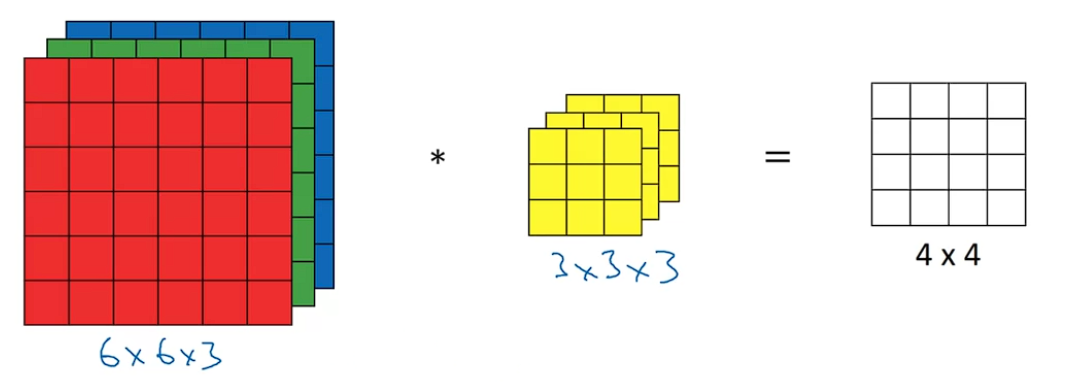
\includegraphics[width=15cm]{23.png}
        \end{figure}
        \item For RGB image, convolutions in each layer are applied then summed together for each pixel
        \begin{itemize}
            \item Filter can be set to detect edges in specific colors or all edges
        \end{itemize}
        \item To detect all edges, vertical filter and horizontal filter can be used
        \begin{itemize}
            \item Outputs from both filters can be stacked over each other
        \end{itemize}
        \item Single layer in a convolutional NN will add a bias term and non-linearity to each output
        \begin{itemize}
            \item Same bias term will be added to all pixels in the image
        \end{itemize}
        \item If using 10 $3\times 3\times 3$ filters, total parameters will be 280
        \begin{itemize}
            \item Number of parameters is independent of the size of the input
            \item Makes CNN less prone to overfitting than standard NN
        \end{itemize} 
        \item For a convolution layer $l$:
        \begin{itemize}
            \item $f^{[l]}$ = filter size
            \item $p^{[l]}$ = padding
            \item $s^{[l]}$ = stride
            \item Input: $n_H^{[l-1]} \times n_W^{[l-1]} \times n_C^{[l-1]}$
            \item Output: $n_H^{[l]} \times n_W^{[l]} \times n_C^{[l]}$
            $$n_H^{[l]}=\left\lfloor\frac{n_H^{[l-1]}+2p^{[l]}-f^{[l]}}{s^{[l]}}+1\right\rfloor$$
            \item Filter: $f^{[l]} \times f^{[l]} \times n_C^{[l-1]}$
            \item Activations:  $a^{[l]} \rightarrow n_H^{[l]} \times n_W^{[l]} \times n_C^{[l]}$ 
            \begin{itemize}
                \item[] $A^{[l]} \rightarrow m \times n_H^{[l]} \times n_W^{[l]} \times n_C^{[l]}$
            \end{itemize}
            \item Weights: $f^{[l]} \times f^{[l]} \times n_C^{[l-1]} \times n_C^{[l]}$
            \item Bias: $n_C^{[l]}$
        \end{itemize}
        \item Each layer in a CNN can have different sizes for padding, filters and stride length
        \begin{itemize}
            \item A lot of the work for CNNs is choosing the hyperparameters for each layer in the network
        \end{itemize}
        \item Final output from the CNN can be unrolled and fed to a logistic regression unit to make a prediction
        
        \item In a CNN, will have convolution layers, pooling layers and fully connected layers
        \item Pooling layers reduce the size of the representation and can make detected features more robust
        \begin{itemize}
            \item Max pooling splits the input into sections and takes the maximum value from each section
            \item Max pooling will have a filter size and stride length
            \item Max pooling will ``preserve'' any standout features 
        \end{itemize}
        \item For a 3D input to max pooling, output will have the same 3rd dimension
        \begin{itemize}
            \item Computation will be applied to each channel separately 
        \end{itemize}
        \item Average pooling takes the average from each filter
        \begin{itemize}
            \item Not as commonly used as max pooling
        \end{itemize}
        \item Padding size of 0 usually used for pooling layers
        \item A fully connected layer is the same as a layer in a standard neural network 
        \begin{itemize}
            \item FC layer will have $W$ and $b$ parameters
            \item Will reduce the dimension of the output of the NN
        \end{itemize}
        \item Further in the CNN, the height and width of the input will gradually decrease
        \begin{itemize}
            \item As $n_W$ and $n_H$ decrease, the depth of the input will typically increase
        \end{itemize}
        \item Typical CNN will have one or more conv layers followed by a pool layer
        \begin{itemize}
            \item CNN will usually finish with some fully connected layers then a softmax layer
        \end{itemize}
        \item Conv layers help the network with sparsity of connections
        \begin{itemize}
            \item Using a $32\times 32\times 3$ input image, 6 filters ($f=5$) will give around 14m parameters 
            \item Conv layer will have 456 parameters for same calculation
            \item In every layer, each output value is depends on only a small number of inputs
        \end{itemize}
        \item Conv layers use parameter sharing
        \begin{itemize}
            \item A feature detector (filter) that is useful in one part of an image will likely be useful in another part of the image
        \end{itemize}
        \item Conv layers and FC layers all have associated parameters
        \begin{itemize}
            \item Cost function can be defined over the parameters
            \item Gradient descent or other optimization algorithm can be used to train the network and reduce J
        \end{itemize}
    \end{itemize}
    \subsection{Deep Convolutional Models: Case Studies}
    \begin{itemize}
        \item Intuition about own deep learning problem can be gained by looking at existing research
        \begin{itemize}
            \item NN architecture and other ideas may be transferrable to other problems
            \item Ideas may also be transferrable to other areas of machine learning
        \end{itemize}
    \end{itemize}
    \subsubsection{LeNet-5}
    \begin{itemize}
        \item Goal of LeNet-5 was to recognize handwritten digits
        \item NN was trained on grayscale images ($32\times 32 \times 1$)
    \end{itemize}
    \begin{figure}[ht]
        \centering
        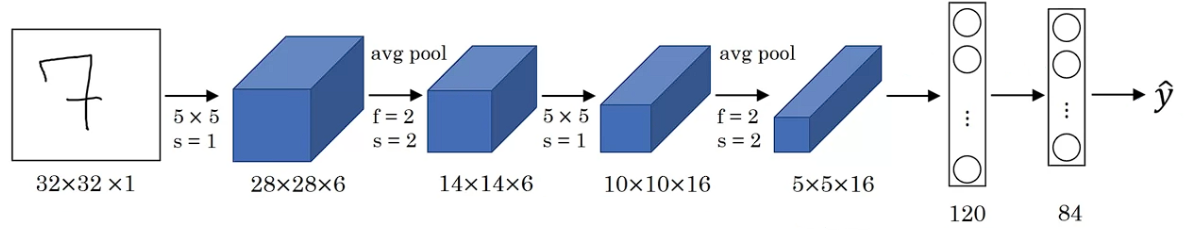
\includegraphics[width=16cm]{24.png}
    \end{figure}
    \begin{itemize}
        \item Output from the NN had 10 possible values 
        \begin{itemize}
            \item Modern implementation would use a softmax layer
        \end{itemize}
        \item When the NN was implemented, no padding was used 
        \item LeNet-5 was ``small'' compared to other networks
        \begin{itemize}
            \item Whole NN had 60K parameters
            \item Modern NN can have 10m to 100m parameters
        \end{itemize}
        \item Deeper in the network, $n_H$ and $n_W$ decrease and $n_C$ increase
        \item Network starts with conv and pool layers, followed by FC layers then output 
        \item Modern computers have the capacity for each filter to have the same number of channels as its input
        \begin{itemize}
            \item LeNet-5 had a method of making different filters looking at different inputs
        \end{itemize}
        \item LeNet-5 used sigmoid or tanh activation functions
        \begin{itemize}
            \item Non linearity was also added after the pooling layers
        \end{itemize}
    \end{itemize}

    \subsubsection{AlexNet}
    \begin{itemize}
        \item Input was a $227\times 227$ color image
        \begin{figure}[ht]
            \centering
            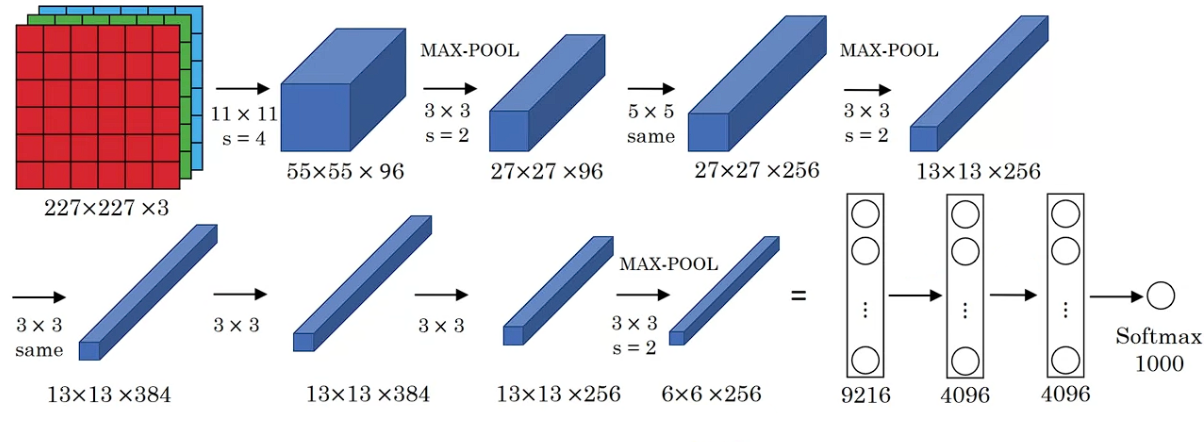
\includegraphics[width=16cm]{25.png}
        \end{figure}
        \item Similar structure to LeNet-5 but much larger
        \begin{itemize}
            \item Contains around 60m parameters
        \end{itemize}
        \item Used ReLU activation functions 
        \item Training of AlexNet was split across multiple GPUs
        \item AlexNet used a Local Response Normalization layer
        \begin{itemize}
            \item After some layers, the outputs would be normalized across all the channels
            \item Not used very often as research showed layer is not very helpful 
        \end{itemize}
    \end{itemize}

    \subsubsection{VGG-16}
    \begin{itemize}
        \item Uses a much simpler network compared to AlexNet
        \begin{itemize}
            \item Conv layers: $3\times 3$ filter, $s=1$, same padding
            \item Max pool layers: $2\times 2$ filter, $s=2$
        \end{itemize}
        \item NN has 16 layers with weights
        \begin{itemize}
            \item NN has around 138m weights
        \end{itemize}
        \begin{figure}[ht]
            \centering
            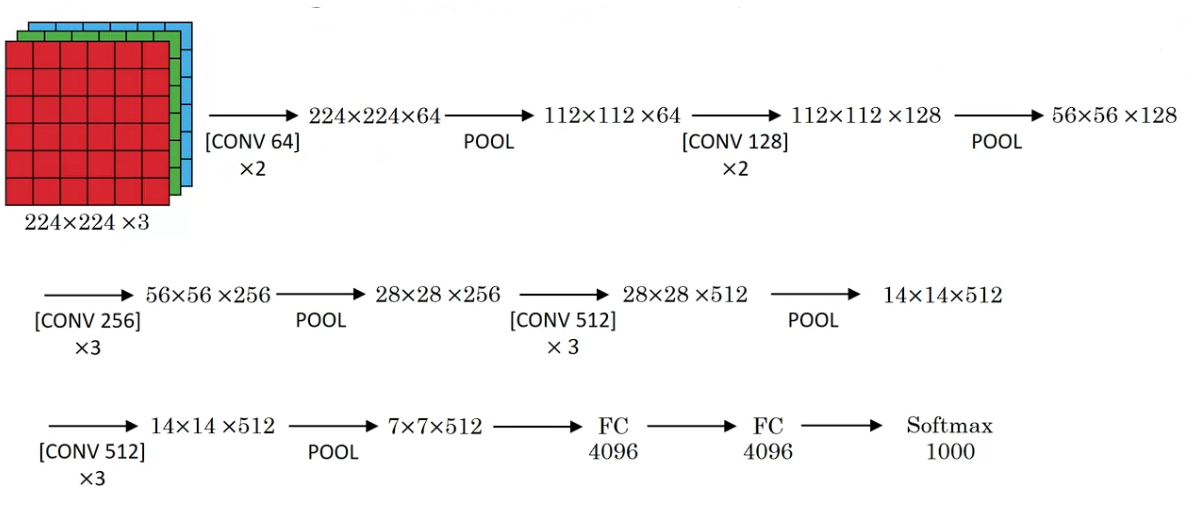
\includegraphics[width=16cm]{26.png}
        \end{figure}
        \item NN is much more uniform when compared with other architectures
    \end{itemize}

    \subsubsection{ResNets}
    \begin{itemize}
        \item Very deep networks are hard to train due to vanishing and exploding gradients
        \item Skip connections use activations from one layer in another layer deeper in the NN
        \item ResNets created by using a residual block
        \begin{itemize}
            \item In between $a^{[l]}$ and $a^{[l+2]}$, the activations $a^{[l]}$ will go through two sets of linear and non linear functions
            \item $a^{[l]}$ can be added later in the network before the second non-linearity
        \end{itemize}
        $$a^{[l+2]}=g(z^{[l+2]}+a^{[l]})$$
        \item  Residual blocks can be stacked together to form a deep network
        \begin{itemize}
            \item Residual blocks allow deeper NN to be trained
        \end{itemize}
        \item For ``plain'' NN, increasing the number of layers will initially decrease the training error
        \begin{itemize}
            \item When the number of layers is very large, the NN is hard to train and the training error increases
            \item With ResNets, the training error shouldn't increase with the number of layers
        \end{itemize}
        \item Residual blocks can quite easily learn the identity function
        \begin{itemize}
            \item Using the ReLU activation, $a^{[l+2]}=g(W^{[l+2]}a^{[l+1]}+b^{[l+2]}+a^{[l]})$
            \item With regularization, $W$ and $b$ will be close to 0
            \item $\therefore a^{[l+2]}\approx g(a^{[l]})$
            \item Since ReLU activation is used, $a^{[l+2]}\approx a^{[l]}$
        \end{itemize}
        \item If adding residual blocks is similar to using the identity function, the performance of the network will not be affected
        \begin{itemize}
            \item Residual blocks can also learn parameters that are better than the identity function
        \end{itemize}
        \item For ResNets, it is assumed that $z^{[l+2]}$ and $a^{[l]}$ have the same dimensions
        \begin{itemize}
            \item Same convolutions tend to be used for ResNets
            \item If same convolution is not used, $a^{[l]}$ is multiplied by a matrix $W_s$ to create the correct dimension
            \item $W_s$ can have parameters that can be learnt or can be a fixed matrix that adds zero padding
        \end{itemize}
    \end{itemize}

    \subsubsection{Networks in Networks}
    \begin{itemize}
        \item For a single $1\times 1\times 1$ filter, pixels in the image will get multiplied by the filter value
        \begin{itemize}
            \item If the filter has a depth of more than 1, the filter will take the element wise product of all numbers in the slice 
            \item Very similar to a neuron taking all the numbers in a slice as input
        \end{itemize}
        \item Having a $1\times 1$ convolution on an input is the same as having a fully connected NN in each position
        \item Using $1\times 1$ convolutions known as network in network
        \item $1\times 1$ convolutions can be used to shrink the depth of an input
        \begin{itemize}
            \item Pooling layers used to shrink the height and width of the volume
        \end{itemize}
    \end{itemize}

    \subsubsection{Inception Network}
    \begin{itemize}
        \item For CNNs, must choose the size of the filters and order of layers
        \begin{itemize}
            \item Inception network works with multiple choices of filters and layers at the same time
        \end{itemize}
        \item Outputs from all possible choices are stacked on top of each other
        \begin{figure}[ht]
            \centering
            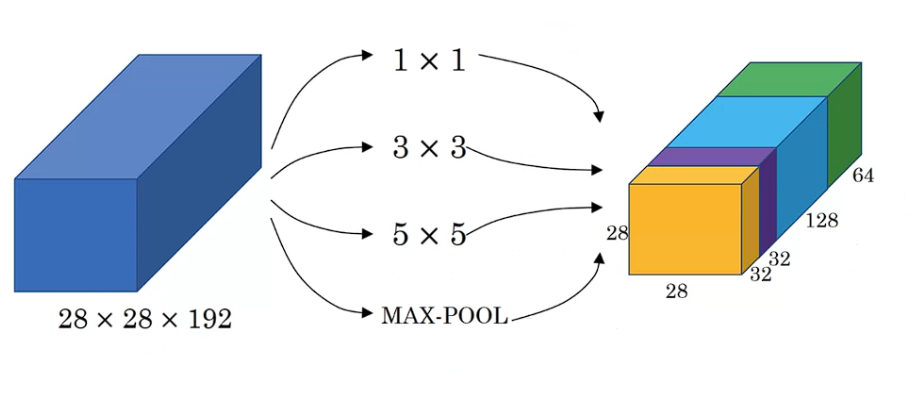
\includegraphics[width=12cm]{27.png}
        \end{figure} 
        \begin{itemize}
            \item Same padding used for conv layers so outputs have the same dimension
            \item Same padding and $s=1$ must also be used for max pooling layer
            \item Output from the layer will be a $28\times 28\times 256$ volume
        \end{itemize}
        \item For the $5\times 5$ filter section of the layer, 120,422,400 calculations are needed
        \begin{itemize}
            \item Single layer of an inception network can be very computationally expensive
            \item $1\times 1$ convolutions can be used to reduce the computational cost by a factor of 10
        \end{itemize}
        \item $1\times 1$ convolutions can be used in a bottleneck layer to shrink the input
        \begin{figure}[ht]
            \centering
            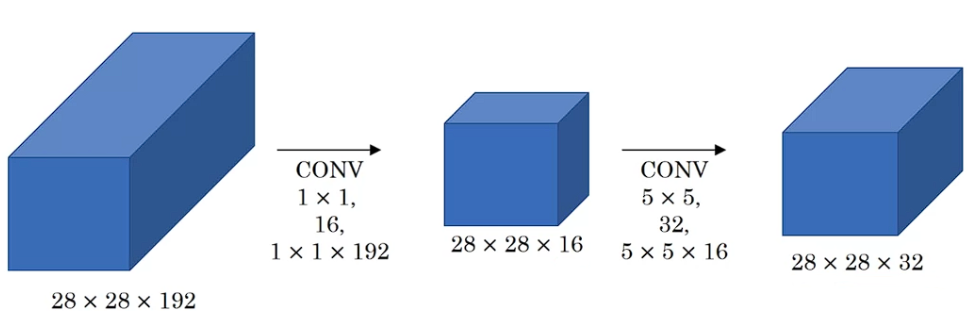
\includegraphics[width=10cm]{28.png}
        \end{figure}
        \begin{itemize}
            \item With the bottleneck layer, only 12,443,648 calculations are needed
        \end{itemize}
        \item For an inception module, $1\times 1$ convolution should be used before any filters that have larger dimensions
        \begin{itemize}
            \item For pooling layers, $1\times 1$ convolutions should be used to shrink the number of channels
        \end{itemize}
        \item Inception network created from multiple inception modules
    \end{itemize}

    \subsubsection{MobileNet}
    \begin{itemize}
        \item MobileNet networks can be built and deployed in low compute environments 
        \begin{itemize}
            \item Can be used for mobile and embedded vision applications due to low computational cost at deployment
        \end{itemize}
        \item For a normal convolution:
        $$\text{Computational cost = \# filter params $\times$ \# filter positions $\times$ \# of filters}$$
        \item A depthwise separable convolution separates process into depthwise and pointwise convolution
        \item Depthwise convolution uses $n_C$ filters of $f\times f$
        \begin{itemize}
            \item Separate filter used for each channel
            \item Output of depthwise convolution will be $n_{out}\times n_{out}\times n_C$
        \end{itemize}
        \item Pointwise convolution uses filters of size $1\times 1\times n_C$
        \begin{itemize}
            \item ${n_C}'$ filters used to get the correct dimensions in the output volume
        \end{itemize}
        \item Computational cost of depthwise and pointwise convolutions will be less than the computational cost for a normal convolution
        \begin{itemize}
            \item In general, the ratio of of computational costs is $\frac{1}{{n_C}'}+\frac{1}{f^2}$
        \end{itemize}
        \item MobileNet will use a depthwise separable convolution for all convolutions in the network
        \begin{itemize}
            \item Original MobileNet V1 network had 13 depthwise separable convolutions
            \item Last layers of the network were pooling, FC and softmax layers 
        \end{itemize}
        \item MobileNet V2 used residual connections across each layer
        \begin{itemize}
            \item Convolution also added an expansion layer before the depthwise convolution 
            \item MobileNet V2 had 17 convolution (bottleneck) blocks with pooling, FC and softmax layers
        \end{itemize}
        \item Expansion layer similar to the pointwise convolution (projection) but increases the depth of the volume
        \begin{itemize}
            \item The expansion increases the size of the representation to allow the NN to learn a richer function
            \item The projection reduces the depth of the volume to reduce the amount of memory required for the output
        \end{itemize}
    \end{itemize}

    \subsubsection{EfficientNet}
    \begin{itemize}
        \item Specific application can benefit from being scaled to the hardware specifications
        \item To scale a NN:
        \begin{itemize}
            \item Higher resolution image
            \item Change the depth of the network
            \item Change the width of the layers
        \end{itemize} 
        \item $r,d,w$ can be scaled according to available resources
        \begin{itemize}
            \item Rate of scaling for each variable may not be the same
        \end{itemize}
    \end{itemize}

    \subsubsection{Practical Advice for CNNs}
    \begin{itemize}
        \item A lot of details about CNNs are hard to replicate in practice
        \begin{itemize}
            \item Open source implementation of code can often be found online 
            \item Reimplementing the whole algorithm from scratch can help in terms of understanding
        \end{itemize}
        \item Specific architecture may also take a very long time to train on own device 
        \begin{itemize}
            \item Transfer learning can be used from pre trained networks
        \end{itemize}
        \item When using a pre trained network, softmax layer can be replaced to suit new application
        \begin{itemize}
            \item Parameters in the rest of the network can be ignored and softmax output layer can be trained
            \item If only the last layer is being trained, the activations input to the softmax layer can be saved separately to prevent extra computation
        \end{itemize}
        \item If the training set is very big, more layers from the end of the network can be trained
        \begin{itemize}
            \item Weights from original network can be used for initialization
            \item Layers can also be completely removed and trained again from the start
            \item Whole network can be retrained if there is enough data
        \end{itemize}
        \item Most computer vision tasks can benefit from data augmentation
        \item Mirroring and random cropping are commonly used for data augmentation
        \begin{itemize}
            \item Mirroring images works well for most applications
            \item Random cropping works well as long as the crop is a reasonable subset of the image 
        \end{itemize}
        \item Other methods can be used but can be less effective
        \begin{itemize}
            \item Rotation
            \item Shearing
            \item Local warping
        \end{itemize}
        \item Color shifting can be used in almost all computer vision applications
        \begin{itemize}
            \item Can help to eliminate any biases caused by specific lighting
            \item In practice, color shifting will be more structured (PCA color augmentation)
        \end{itemize}
        \item When training, a specific CPU thread will be used to apply distortions
        \begin{itemize}
            \item The data will be processed by the thread then passed to the CPU/GPU for training
            \item CPU thread for distortion and CPU for training can run in parallel
        \end{itemize}
        \item Some applications of deep learning have comparatively more data than other applications
        \begin{itemize}
            \item Speech recognition has a lot of available labelled data
            \item Image recognition has a lot of data but not ``enough'' for applications
            \item Object detection had relatively little labelled data
        \end{itemize}
        \item Applications with comparatively more data can use simpler algorithms
        \begin{itemize}
            \item Applications with comparatively less data require more hand engineering of features 
        \end{itemize}
        \item Historically, computer vision relies more on hand engineered features
        \begin{itemize}
            \item Network architectures are also hand engineered for computer vision
        \end{itemize}
        \item Researchers also want to do well on benchmarks and win ML competitions
        \begin{itemize}
            \item Some researchers will use ideas that will specifically help the benchmark
            \item Same ideas would not be used in a standard application 
        \end{itemize}
        \item Ensembling can give a slight increase to the performance of an algorithm
        \begin{itemize}
            \item Several networks are trained independently and the outputs are averaged
            \item 3-15 networks can be used but will greatly slow down the running time
        \end{itemize}
        \item Multi-crop at test time is more computationally expensive and much slower
        \begin{itemize}
            \item The trained classifier is run on multiple versions of test images and results are averaged
            \item 10-crop applies same network to 10 separate crops of the image
        \end{itemize}
    \end{itemize}

    \subsection{Object Detection}
    \begin{itemize}
        \item Image classification identifies whether an object is contained within an image
        \begin{itemize}
            \item Classification with localization will identify the location of the object on the image
            \item Detection will search and locate multiple objects in an image
        \end{itemize}
        \item For classification with localization, output of the NN will typically include a softmax output
        \begin{itemize}
            \item Output layer must also be modified to output the coordinates for the bounding box ($b_x, b_y, b_w, b_h$)
        \end{itemize}
        \item For a 4 class localization problem:
        $$y=\begin{bmatrix}
            P_c \\
            b_x \\
            b_y \\
            b_h \\
            b_w \\
            c_1 \\
            c_2 \\
            c_3 \\
        \end{bmatrix}$$
        \begin{itemize}
            \item $P_c$: 1 if an object has been identified
            \item $b_x, b_y, b_h, b_w$: coordinates for the bounding box
            \item $c_1, c_2, c_3$: class labels for 3 positive classes
        \end{itemize}
        $$\mathcal{L}(\hat{y}, y)=\begin{cases}
            (\hat{y_1}-y_1)^2+(\hat{y_2}-y_2)^2+...+(\hat{y_8}-y_8)^2,&\text{if $y_1$=1} \\
            (\hat{y_1}-y_1)^2,&\text{if $y_1$=0}
        \end{cases}$$
        \item In practice, feature loss for softmax output or logistic regression loss is used
        \item NNs can be trained to output coordinates for landmarks in the image
        \begin{itemize}
            \item Training set must be labelled with all the landmarks on the image
        \end{itemize}
        \item Landmark detection can be used for AR filters or to track emotions and poses
        \item Object detection with CNNs can be done with a sliding windows detection algorithm
        \begin{itemize}
            \item Training set should contain closely cropped images of wanted object
            \item CNN can be trained to output label for closely cropped image
            \item Trained CNN passed to the sliding windows classifier
        \end{itemize}
        \item For sliding windows classifier, specific window size is chosen and overlayed on the image
        \begin{itemize}
            \item Section of image in the window passed to the trained CNN
            \item Window ``slides'' across the whole image 
            \item After initial pass of image is made, a larger window size is used
        \end{itemize}
        \item Sliding windows detection is very computationally expensive
        \begin{itemize}
            \item A coarser stride can be used to reduce computational load
            \item Larger stride length can damage the algorithm performance
            \item Initial classifiers used, simpler classifiers with hand engineered features
        \end{itemize}
        \item Convolutional implementation of the sliding windows detection is more computationally feasible
        \item FC layers can be transformed into convolutional layers
        \begin{itemize}
            \item For a input of $5\times 5\times 16$ to a FC layer, a $5\times 5$ filter can be used
            \item 400 filters must be used for output to have the correct dimension
            \item Softmax output can be seen as a $1\times 1\times n_{Cout}$ volume
        \end{itemize}
        \item Once the initial CNN is trained, the network can be run on the whole image
        \begin{itemize}
            \item Output from the image will be a volume that represents all the possible inputs to the CNN
            \item Only requires forward propagation to be run once as computation is shared
        \end{itemize}
        \item Using convolutional implementation, bounding boxes still may not be very accurate
        \begin{itemize}
            \item Discrete steps may not match up exactly with the object
            \item Object may be more rectangular in the image
        \end{itemize}
        \item YOLO algorithm will increase the accuracy of the bounding boxes
        \begin{itemize}
            \item Image is split into grid and object classifier run on each cell
            \item Any located objects assigned to the cell containing the midpoint
            \item Using above output and a $3\times 3$ grid, target output will be $3\times 3\times 8$
            \item CNN should be chosen so that output is also $3\times 3\times 8$
        \end{itemize}
        \item Trained network will give precise bounding boxes for each cell
        \begin{itemize}
            \item Each cell cannot have more than a single object
            \item For a fine grid, the chances of having more than one object in each cell is low
            \item Algorithm is fast enough for real time object detection
        \end{itemize}
        \item When specifying the coordinates for the bounding box, $b_x$ and $b_y$ should be relative to their cell
        \begin{itemize}
            \item $b_h$ and $b_w$ should be a fraction of the cell dimensions
            \item $b_h$ and $b_w$ can be larger than 1
        \end{itemize}
        \item Intersection over union can be used to evaluate an object detection algorithm
        \begin{itemize}
            \item Calculates the quotient of the intersection and union for the ground truth and predicted bounding box
            \item May CV tasks judge the answer as correct if IoU $\geq 0.5$ 
        \end{itemize}
        \item Non-max suppression ensures the algorithm only detects each object once
        \begin{itemize}
            \item With the YOLO algorithm, more than one box may think it has the center of the object  
        \end{itemize}
        \item Algorithm starts by discarding rectangles with $p_c \leq0.6$
        \begin{itemize}
            \item Rectangle with the larges $p_c$ is chosen as prediction
            \item Any other boxes with IoU $\geq0.5$ can be discarded
        \end{itemize}
        \item Non-max suppression should be carried out on each of the output classes
        \item Anchor boxes can be used to allow cells to detect multiple objects
        \begin{itemize}
            \item Shapes for anchor boxes can be defined for possible objects in the image
            \item Output vector $y$ will have a vector for each anchor box
            \item Each object is assigned to the grid cell that contains the midpoint and anchor box that has the highest IoU
        \end{itemize}
        \begin{figure}[ht]
            \centering
            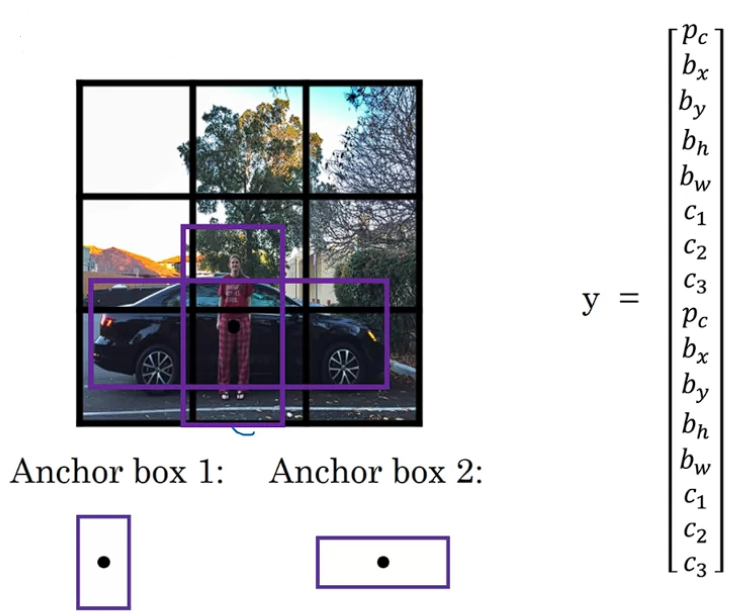
\includegraphics[width=10cm]{29.png}
        \end{figure}
        \item If there are more objects than anchor boxes, alternative case should be implemented in the algorithm
        \item Anchor boxes allow the algorithm to better specialize to certain objects
        \begin{itemize}
            \item K means algorithm can be used to group together object shapes that get detected
        \end{itemize}
        \item To train YOLO algorithm, all images in the training set must be properly labelled
        \begin{itemize}
            \item For each image, the output $y$ will be a volume with the vector $y$ for each cell
            \item For each class, non-max suppression used to generate final predictions
        \end{itemize}
        \item Convolutional object classifiers will get run on all parts of the image
        \begin{itemize}
            \item Some areas of the image clearly do not have any object in them
            \item R-CNN will use a segmentation algorithm to propose regions that likely have objects in them
            \item All proposed regions run through the object classifier
        \end{itemize}
        \item R-CNN still a relatively slow algorithm
        \begin{itemize}
            \item Fast R-CNN uses a convolutional implementation to classify the proposed regions 
            \item Faster R-CNN uses a CNN to propose the regions 
        \end{itemize}
        \subsubsection{U-Nets}
        \item Semantic segmentation aims to identify an outline of any identified objects
        \begin{figure}[ht]
            \centering
            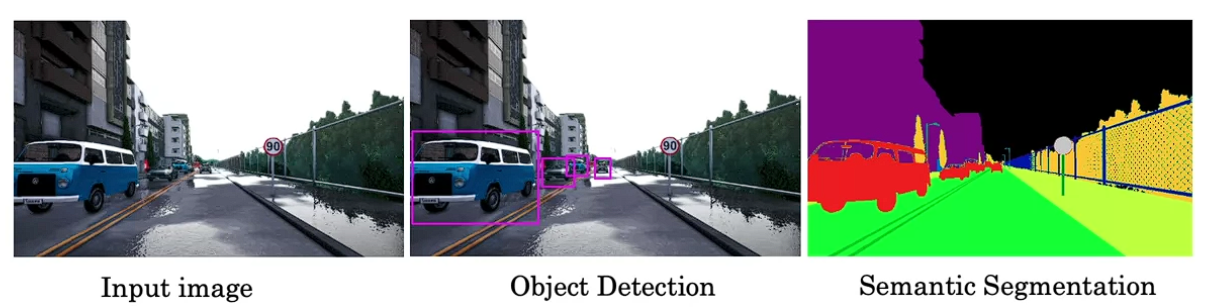
\includegraphics[width=16cm]{30.png}
        \end{figure}
        \begin{itemize}
            \item Used by some self driving car teams to detect drivable roads
            \item Used by medical teams to help with reading scans
            \item Segmentation done with a U-Net
        \end{itemize}
        \item U-Net has to generate a matrix of labels for each image to segment each pixel
        \begin{itemize}
            \item First few layers of standard CNN can be reused
            \item Last few layers of the CNN must make the output the same size as the input
            \item Transpose convolution must be used to increase the height and width of each layer
        \end{itemize}
        \item Regular convolution will place filter on top of the input
        \begin{itemize}
            \item Transpose convolution will put the filter on top of the output
        \end{itemize}
        \item For each value in the input, filter gets multiplied by the input and overlayed on the output
        \begin{itemize} 
            \item Numbers for each filter get added to the output values
            \item Values in the padding can be ignored
        \end{itemize}
        \item For the U-Net architecture, skip connections can be used to improve performance
        \begin{itemize}
            \item When the dimensions of the layers decrease in the CNN, spatial information is lost
        \end{itemize}
        \begin{figure}[ht]
            \centering 
            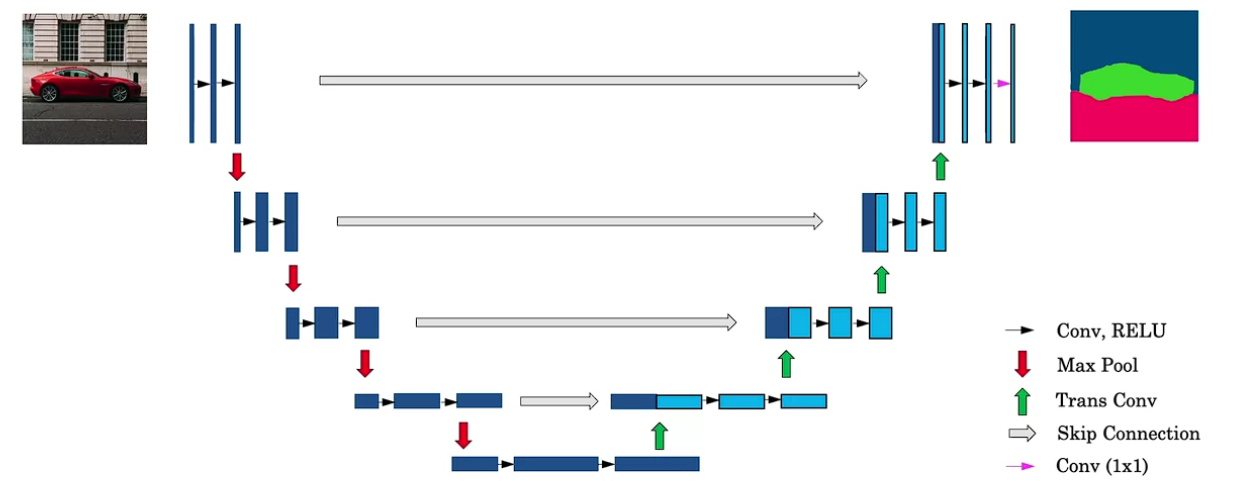
\includegraphics[width=16cm]{31.png}
        \end{figure}
        \item Conv and ReLU layers will increase number of channels in the image 
        \begin{itemize}
            \item Height and width will remain unchanged  
        \end{itemize}
        \item Max pool layers will decrease the height and width of the image
        \begin{itemize}
            \item Number of channels will remain constant
        \end{itemize}
        \item After transpose convolutions are used, corresponding conv layer will use a skip connection
        \item Last layer will be a $1\times 1$ convolution
        \item Dimension of last layer will be $h\times w\times n_{classes}$
    \end{itemize}

    \subsection{Special Applications of CNNs}
    \subsubsection{Face Recognition}
    \begin{itemize}
        \item Face recognition can be paired with liveness detection to distinguish real faces from images
        \item Face verification takes an input image and an ID
        \begin{itemize}
            \item Output will state if the input image is the same as the ID
        \end{itemize}
        \item Face recognition will take an input image and compare it to $K$ different people
        \begin{itemize}
            \item Output will give the ID of any recognized person
        \end{itemize}
        \item Face verification system may have a very low 1\% error rate
        \begin{itemize}
            \item If the system is used fro face recognition with a database of 100 people, error will be very high 
        \end{itemize}
        \item Majority of face recognition systems must be able to recognize a person from a single example (one-shot learning problem)
        \begin{itemize}
            \item Deep learning problems don't tend to work well with a single example   
        \end{itemize}
        \item Standard CNN with softmax output won't be able to learn well 
        \begin{itemize}
            \item If another person is added to the database, the whole CNN must be retrained
        \end{itemize}
        \item Face recognition functions will learn a similarity function to output the degree of difference between images
        \begin{itemize}
            \item If $d(\text{img1, img2})\leq \tau$ the images are the ``same''
        \end{itemize}
        \item Similarity function will be run on all images in the database
        \item Siamese network can be used to create the similarity function
        \begin{itemize}
            \item Standard CNN ends with a feature vector being fed to a softmax unit
            \item Final layer of the CNN can be seen as an encoding of the input image $x^{(1)}$
            \item Siamese network runs the same CNN network on two inputs and compares the output
        \end{itemize}
        \item Difference between the images can be calculated as the norm between the 2 vectors: 
        $$d(x^{(1)}, x^{(2)})=||f(x^{(1)})-f(x^{(2)})||^2$$
        \item Parameters of the CNN define the encoding $f(x^{(i)})$
        \begin{itemize}
            \item If $x^{(i)}$ and $x^{(j)}$ are the same person, $||f(x^{(i)})-f(x^{(j)})||^2$ should be small
            \item If $x^{(i)}$ and $x^{(j)}$ are different people, $||f(x^{(i)})-f(x^{(j)})||^2$ should be large
        \end{itemize}
        \item Parameters of the CNN can be learnt by using gradient descent on the triplet loss function
        \begin{itemize}
            \item Triplet loss will look at an anchor image, positive image and negative image
            \item Want $d(A,P)\leq d(A,N)$
        \end{itemize}
        \item Loss function can have a trivial solution where all encodings get output to 0
        $$||f(A)-f(P)||^2-||f(A)-f(N)||^2+\alpha\leq 0$$
        \begin{itemize}
            \item Adding constant $\alpha$ prevents the trivial solution from being learnt
        \end{itemize}
        $$\mathcal{L}(A,P,N)=\max(||f(A)-f(P)||^2-||f(A)-f(N)||^2+\alpha, 0)$$
        $$J=\sum_{i=1}^m\mathcal{L}(A^{(i)}, P^{(i)}, N^{(i)})$$ 
        \item Training the system requires sets of anchor, positive and negative images
        \item During training, if $A,P,N$ are chosen randomly, loss function is easily satisfied
        \begin{itemize}
            \item Ideally, chosen triplets should be ``hard'' to train on ($d(A,P)\approx d(A,N)$)
        \end{itemize}
        \item Large scale face recognition systems can be trained on datasets with 10,000,000+ images
        \item Face recognition can also be seen as a binary classification problem
        \begin{itemize}
            \item Outputs from the siamese networks can be fed to a logistic regression unit
            \item Training set will require pairs of images
        \end{itemize}
        $$\hat{y}=\sigma\left(\sum_{k=1}^{128}w_k|f(x^{(i)})_k-f(x^{(j)})_k|+b\right)$$
        \item Different formula can be used to combine both outputs
        \begin{itemize}
            \item Chi Squared similarity
        \end{itemize}
        $$\frac{\left(f(x^{(i)})_k-f(x^{(j)})_k\right)^2}{f(x^{(i)})_k+f(x^{(j)})_k}$$
        \item With Siamese networks, values can be precomputed for stored images
    \end{itemize}

    \subsubsection{Neural Style Transfer}
    \begin{itemize}
        \item Neural style transfer allows existing content to be generated in a different style
        \item To visualize the learning of a CNN, can manually look for image patches that maximize the unit's activation
        \begin{itemize}
            \item First layers of the network will detect simple patterns or colors
            \item Deeper layers will detect more complex patterns and will start to detect certain objects
        \end{itemize}
        \item Cost function can be defined to see how ``good'' an image is
        $$J(G)=\alpha J_{content}(C,G)+\beta J_{style}(S,G)$$
        \item The new image $G$ will be first initialized randomly
        \begin{itemize}
            \item Use gradient descent to minimize $J(G)$
            \item Gradient descent will change the pixel values of the image
        \end{itemize}
        \item A layer $l$ will be chosen to compute the content cost
        \begin{itemize}
            \item If the layer $l$ is too shallow, the pixel values are forced to be very close to the content image
            \item If the layer $l$ is too deep, the content may be too dissimilar
        \end{itemize}
        \item Using a pre trained CNN, activations of the images on layer $l$ can be calculated
        \begin{itemize}
            \item If $a^{[l](c)}$ and $a^{[l](G)}$ are similar, both images have similar content
        \end{itemize}
        $$J_{content}(C,G)=\frac{1}{2}\left|\left|a^{[l](C)}-a^{[l](g)}\right|\right|^2$$
        \item The style of a layer can be calculated as the correlation between activations across different channels
        \begin{itemize}
            \item All pixels can be compared with the corresponding pixel in a different channel
            \item A single pixel will have a specific pattern that results in high activation
            \item Correlation between the layers show which patterns tend to occur together
        \end{itemize}
        \item Style matrix can be defined:
        \begin{itemize}
            \item Let $a_{i,j,k}^{[l]}$ be the activation of layer $l$ at $(i,j,k)$
            \item $G^{[l]}$ is a $n_c^{[l]}\times n_c^{[l]}$ matrix 
            $$G^{[l](G)}_{k~k'}=\sum_{i=1}^{n_H^{[l]}}\sum_{j=1}^{n_w^{[l]}}a^{[l](G)}_{i,j,k}~a^{[l](G)}_{i,j,k'}$$
            \item $G$ is calculated for all values of $k$ and $k'$ for the style image and generated image
        \end{itemize}
        \item Style cost function is then the difference between the style matrices
        \begin{align*}
            J_{style}^{[l]}(S,G)&=\left|\left|G^{[l](S)}-G^{[l](G)}\right|\right|^2_F \\
            &=\frac{1}{\left(2n_H^{[l]}n_W^{[l]}n_C^{[l]}\right)^2}\sum_k\sum_{k'}\left(G_{k~k'}^{[l](S)}-G_{k~k'}^{[l](G)}\right)^2
        \end{align*}
        \begin{itemize}
            \item Constant comes from original authors of the paper
            \item Constant will be superseded by the constant in the overall style transfer const function
        \end{itemize}
        \item Performance is increased when the style cost function is taken from multiple layers
        $$J_{style}(S,G)=\sum_l\lambda^{[l]}J_{style}^{[l]}(S,G)$$
        \begin{itemize}
            \item Using all layers of the CNN allows all levels of features to be used
        \end{itemize}
        \item Convolutions can also be applied to 1D data
        \begin{itemize}
            \item ECG data can be convolved with a 1D filter
            \item CT scans can be convolved with a 3D filter
        \end{itemize}
    \end{itemize}
    \pagebreak

    \section{Sequence Models}
    \subsection{Recurrent Neural Networks}
    \begin{itemize}
        \item Sequence models work with different types of sequence data
        \begin{itemize}
            \item Speech recognition: input and output both sequence data
            \item Music generation: output is sequence data, input can be multiple types (also $\emptyset$)
            \item Sentiment classification: input is sequence data, output is usually categorical
            \item DNA sequence analysis: input and output both sequence data
            \item Machine translation: input and output both sequence data
            \item Video activity recognition: input is sequence data
            \item Name entity recognition: input is sequence data 
        \end{itemize} 
        \item Name entity recognition used by search engines to index entities from text
        \begin{itemize}
            \item Input will be a sequence of words
            \item Output can be a list of numbers corresponding to each word in the sequence
        \end{itemize}
        \item For sequence data:
        \begin{itemize}
            \item $x^{(i)<t>}$: $t^{th}$ element in example $i$
            \item $y^{(i)<t>}$: $t^{th}$ element in example $i$
            \item $T_x^{(i)}$: length of the input for example $i$
            \item $T_y^{(i)}$: length of the output for example $i$
        \end{itemize}
        \item NLP applications will have a dictionary of known words
        \begin{itemize}
            \item Dictionary can come from most common words in training set or from online sources  
        \end{itemize}
        \item One-hot representation can be used for words in the sequence data
        \begin{itemize}
            \item Each word will be a vector of the same length as the dictionary
        \end{itemize}
        \item Standard network taking one hot vectors as input doesn't work well in practice
        \begin{itemize}
            \item For different examples, inputs and outputs can be different lengths
            \item Standard NN won't share features learned across different positions of text 
            \item Standard NN would have large numbers of parameters in hidden layers 
        \end{itemize}
        \item A recurrent neural network takes each input into a layer one at a time
        \begin{itemize}
            \item Outputs of each layer passed to the next instance of the layer
            \item First layers will have a vector of 0s
        \end{itemize}
        \item Parameters for each time step are shared
        \begin{itemize}
            \item $W_{aa}$ for the horizontal activations between layers
            \item $W_{ax}$ for the input to the each layer
            \item $W_{ya}$ for the output predictions
        \end{itemize}
        \item Version of RNN can only use information from previous words
        \begin{figure}[ht]
            \centering
            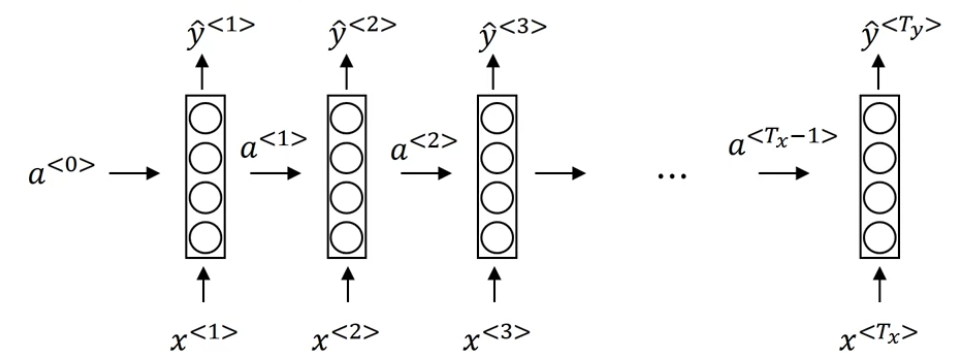
\includegraphics[width=10cm]{32.png}
        \end{figure}
        $$a^{<t>}=g(W_{aa}a^{<t-1>}+W_{ax}x^{<t>}+b_a)$$
        $$\hat{y}^{<t>}=g(W_{ya}a^{<t>}+b_y)$$
        \begin{itemize}
            \item For parameters, first letter is the output quantity, second letter is the input quantity
            \item Activation function for the input values is typically tanh or ReLU
            \item Activation function for the prediction depends on the output type
        \end{itemize}
        \item Notation can be simplified to have a single parameter matrix for each equation
        $$W_a=\begin{bmatrix}
            W_{aa} & \mid & W_{ax}
        \end{bmatrix}$$
        $$[a^{<t-1>},~x^{<t>}]=\begin{bmatrix}
            a^{<t-1>} \\
            \text{---} \\
            x^{<t>}
        \end{bmatrix}$$
        $$a^{<t>}=g(W_a[a^{<t-1>},~x^{<t>}]+b_a)$$
        $$\hat{y}^{<t>}=g(W_ya^{<t>}+b_y)$$
        \item Backprop through an RNN will usually be included in a programming framework
        \item Overall loss for RNN is the sum of the individual losses per time step
        $$\mathcal{L}^{<t>}(\hat{y}^{<t>},y^{<t>})=-y^{<t>}\log\hat{y}^{<t>}-(1-y^{<t>})\log(1-\hat{y}^{<t>})$$
        $$\mathcal{L}(\hat{y}, y)=\sum_{t=1}^{T_y}\mathcal{L}^{<t>}(\hat{y}^{<t>},y^{<t>})$$
        \item Most significant calculation comes from the backprop of the activation values
        \item RNN architecture can be modified if $T_x$ and $T_y$ don't match up
        \begin{itemize}
            \item Input and output can be different types (sentiment classification)
            \item Input and output can be the same data type but have different lengths (machine translation)
        \end{itemize}
        \item Many to many architecture works when $T_x$ is the same as $T_y$
        \begin{itemize}
            \item Many to one architecture has a single output in the final time step 
            \item One to many architecture has a single input in the first time step
        \end{itemize}
        \item Many to many architecture must be modified if $T_x$ and $T_y$ are not the same
        \begin{itemize}
            \item RNN split into encoder and decoder to first read all the input then give all the output
        \end{itemize}
        \begin{figure}[ht]
            \centering
            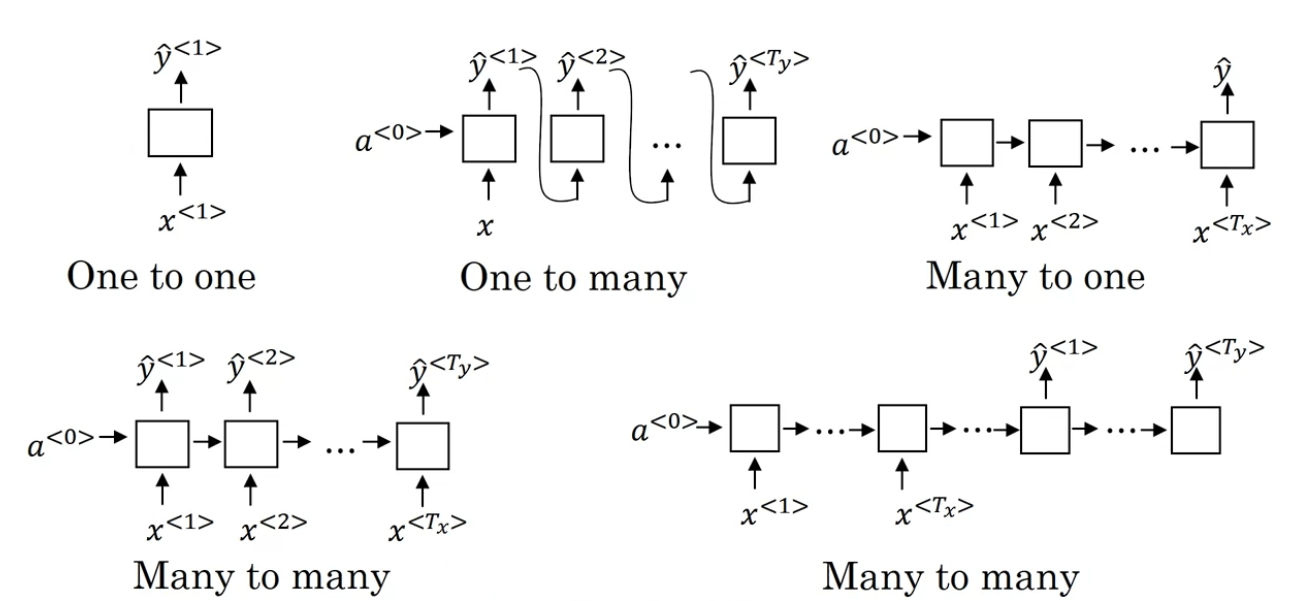
\includegraphics[width=16cm]{33.png}
        \end{figure}
    \end{itemize}
    \subsubsection{Language Modelling}
    \begin{itemize}
        \item RNNs commonly used for language modelling in natural language processing
        \begin{itemize}
            \item Language modelling can be used to distinguish homonyms in sentences
            \item Used in speech recognition and machine translation systems
        \end{itemize}
        \item Given a random sentence, language model will give the probability of a sequence of words
        $$P(y^{<1>}, y^{<2>},y^{<3>},...,y^{T_y})$$ 
        \item Training set for language model requires a large corpus of English text
        \begin{itemize}
            \item Input sentence should first be tokenized
            \item End of the sentence can be marked with a token $<$EOS$>$
            \item Punctuation can be included in the vocabulary and included as tokens
        \end{itemize}
        \item Words that aren't in the dictionary can be replaced with an $<$UNK$>$ token 
        \item RNN model will use a softmax layer to predict the chance of the words in the dictionary
        \begin{itemize}
            \item Softmax layer will have as many outputs as words in the dictionary 
            \item Layer will have outputs for additional tokens as well
            \item First time step will have $a^{<0>}=\overrightarrow{0}$ and $x^{<0>}=\overrightarrow{0}$
        \end{itemize} 
        \item For the second layer, $x^{<2>}=y^{<1>}$
        \begin{itemize}
            \item Layer will try to predict the probability of the second word given the first word
        \end{itemize}
        $$\hat{Y}^{<2>}=P(y^{<2>}|y^{<1>})$$ 
        \item Softmax loss function used to train the RNN for language modelling
        $$\mathcal{L}(\hat{y}^{<t>},y^{<t>})=-\sum_iy_i^{<t>}\log\hat{y}_i^{<t>}$$ 
        $$\mathcal{L}=\sum_t\mathcal{L}^{<t>}(\hat{y}^{<t>},y^{<t>})$$
        \item Once a sequence model has been trained, performance can be gauged by sampling novel sequences
        \begin{itemize}
            \item The output of each layer will be a distribution of probabilities for all possible words
            \item Random sample can be taken over the distribution for each layer
            \item Instead of passing the actual word $y^{<1>}$ to the next layer, $\hat{y}^{<1>}$ is passed instead
        \end{itemize}
        \item Novel sequence can be programmed to reject $<$UNK$>$ token from the sequence
        \item Novel sequence can continue until a $<$EOS$>$ token is predicted
        \begin{itemize}
            \item Length of the novel sequence can also be pre set
        \end{itemize}
        \item Language model can also be made at the character level
        \begin{itemize}
            \item Dictionary would be changed to include letters, punctuation and numbers 
            \item Character level model will not need to include $<$UNK$>$ tokens
            \item Sequences from the character model will be much longer than word level models
        \end{itemize}
        \item English can have very long term dependencies across sentences 
        \begin{itemize}
            \item Basic RNN doesn't do a very good job at capturing long term dependencies
            \item Errors associated with later time steps have a small effect due to vanishing gradients 
            \item Basic RNN model tends to have mainly local influences
        \end{itemize}
        \item Exploding gradients often leads to numerical overflow in the RNN
        \begin{itemize}
            \item Gradient clipping can be used to ``clip'' gradients that are above a chosen threshold
        \end{itemize}
        \item More complex applications may require a deep RNN
        \begin{itemize}
            \item Deep RNNs use a RNN as a single layer in a standard NN
        \end{itemize}
        \item Notation must be modified to distinguish between layers
        \begin{itemize}
            \item $a^{[2]<1>}$ is the first activation in the second layer
            \item Each layer will have its own parameters $W_a^{[l]}$ and $b_a^{[l]}$
        \end{itemize}
        $$a^{[l]<t>}=g(W_a^{[l]}[a^{[l]<t-1>},a^{[l-1]<t>}]+b_a^[l])$$ 
        \item Deep RNN will not have a lot of layers due to computational cost
        \item Output from a deep RNN may be fed to an unconnected deep network
    \end{itemize}
    \subsubsection{Gated Recurent Unit (GRU)}
    \begin{itemize}
        \item GRU modifies the standard RNN layer that helps it to capture long range connections
        \begin{itemize}
            \item Helps with the vanishing gradient problem
        \end{itemize}
        \item The GRU unit will have a variable $c$ for a memory cell
        $$c^{<t>}=a^{<t>}$$
        \item At every time step, unit will consider overwriting the memory cell with $\tilde{c}^{<t>}$
        $$\tilde{c}^{<t>}=\tanh(W_c[\Gamma_r*c^{<t-1>},x^{<t>}]+b_c)$$
        $$\Gamma_u=\sigma(W_u[c^{<t-1>},x^{<t>}]+b_u)$$
        $$\Gamma_r=\sigma(W_r[c^{<t-1>},x^{<t>}]+b_r)$$
        \item The ``gate'' will decide if the memory cell will get updated
        \begin{itemize}
            \item Since sigmoid is used for the gate function, value will likely be close to 0 or 1
        \end{itemize}
        \item $\Gamma_r$ is the relevance of $c^{<t-1>}$
        $$c ^{<t>}=\Gamma_u*\tilde{c}^{<t>}+(1-\Gamma_u)*c^{<t-1>}$$
        \item $c^{<t>},\tilde{c}^{<t>}$ and $\Gamma_u$ will all be the same dimensions
        \begin{itemize}
            \item Element wise multiplication used if values are vectors
        \end{itemize}
    \end{itemize}
    \subsubsection{Long Short Term Memory (LSTM) unit}
    \begin{itemize}
        \item LSTM is a more general version of the GRU
        \begin{itemize}
            \item Memory gate value doesn't have to be the same as the activation values
        \end{itemize}
    \end{itemize}
    $$\tilde{c}^{<t>}=\tanh(W_c[a^{<t-1>},x^{<t>}]+b_c)$$  
    $$\Gamma_u=\sigma(W_u[a^{<t-1>},x^{<t>}]+b_u)$$
    $$\Gamma_f=\sigma(W_f[a^{<t-1>},x^{<t>}]+b_f)$$ 
    $$\Gamma_o=\sigma(W_o[a^{<t-1>},x^{<t>}]+b_o)$$
    $$c^{<t>}=\Gamma_u*\tilde{c}^{<t>}+\Gamma_f*c^{<t-1>}$$ 
    $$a^{<t>}=\Gamma_o*\tanh(c^{<t>})$$
    \begin{figure}[ht]
        \centering 
        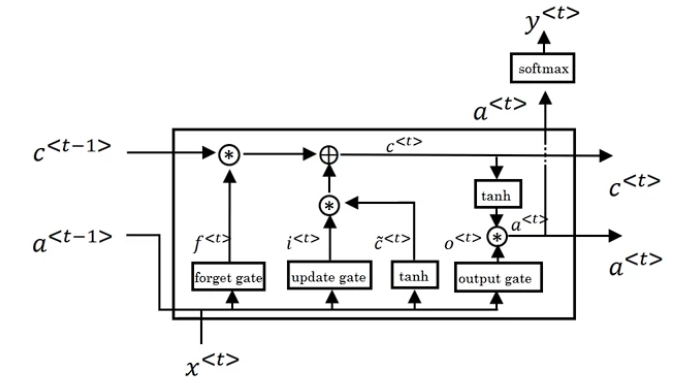
\includegraphics[width=12cm]{34.png}
    \end{figure}
    \begin{itemize}
        \item $a^{<t-1>}$ and $x^{<t>}$ used to calculate each gate
        \item When LSTMs are used in a sequence, values from $c^{<0>}$ can easily pass through each LSTM
        \item Peephole LSTM adds the value of $c^{<t-1>}$ to the matrix in the gate
        \item GRU is a simpler model
        \begin{itemize}
            \item Runs faster and scales to larger models
        \end{itemize}
        \item LSTM is more powerful and flexible than the GRU
    \end{itemize}
    \subsubsection{Bidirectional RNNs (BRNN)}
    \begin{itemize}
        \item Bidirectional RNNs can take information from further ahead in a sequence
        \begin{itemize}
            \item Architecture allows each unit to use information from anywhere in the sequence
        \end{itemize}
        \item Model requires the whole sequence to be read in before being used
        \begin{itemize}
            \item Real time speech recognition models have more complex models that work in real time
        \end{itemize}
        \item BRNN will have both $\overrightarrow{a}^{<t>}$ and $\overleftarrow{a}^{<t>}$ 
        \begin{itemize}
            \item Output $\hat{y}^{<t>}$ from the model will use both $\overrightarrow{a}^{<t>}$ and $\overleftarrow{a}^{<t>}$
        \end{itemize}
        $$\hat{y}^{<t>}=g(W_y[\overrightarrow{a}^{<t>},\overleftarrow{a}^{<t>}]+b_y)$$
        \item For NLP, BRNN with LSTM is commonly used
    \end{itemize}

    \subsection{Natural Language Processing and Word Embeddings}
    \begin{itemize}
        \item Word embeddings allow algorithms to understand analogies in words
        \begin{itemize}
            \item Word embeddings allow NLP applications to be made with relatively small training sets
        \end{itemize}
        \item Words in RNNs represented using a vocabulary of words and one-hot representation
        \begin{itemize}
            \item Representation treats words as separate objects
            \item Algorithm cannot generalize across different words
        \end{itemize}
        \item Featurized representation of words can be created for all words in the dictionary
        \begin{itemize}
            \item Words can then be described in terms of their features instead of the one-hot representation
            \item Featurized representation allows algorithm to make connections between related words 
        \end{itemize}
        \item Learned features for word representation may not have a well defined meaning 
        \item Feature vector for words can be visualized in 2D using the t-SNE algorithm
        \item Word embeddings will help with named entity recognition
        \begin{itemize}
            \item Algorithm will be able to generalize better to structures it has seen before 
        \end{itemize}
        \item Algorithms to learn word embeddings can work with very large text corpuses
        \begin{itemize}
            \item Initial model can be trained with large corpus with 1b-100b words
            \item Transfer learning can then be used for NLP application with a smaller dataset
        \end{itemize}
        \item Word embedding representation will be much smaller than the one-hot representation
        \begin{itemize}
            \item Word embedding representation will be a much smaller vector but a lot more dense 
        \end{itemize}
        \item Difference between words in word embeddings allows algorithms to learn analogies
        \begin{itemize}
            \item The vectors $e_{man}-e_{woman}$ and $e_{king}-e_{queen}$
        \end{itemize}
        \item Given a word pair, algorithm can search the dictionary for the most similar word pair
        $$\mathop{\text{maximize}}_{\textbf{w}}~~\text{sim}(e_w,e_{king}-e_{man}+e_{woman})$$
        \item Cosine similarity commonly used for similarity function
        $$\text{sim}(u,v)=\frac{u^Tv}{||u||_2||v||_2}$$
        \item Euclidean distance between vectors can also be used
        \begin{itemize}
            \item Distance calculated the ``dissimilarity'' between vectors so the negative should be taken
        \end{itemize}
        \item Embedding matrix will be learned to represent all the words in the dictionary
        \begin{itemize}
            \item Product of embedding matrix and one hot representation of a word gives the word embedding representation
        \end{itemize}
        $$E\times O_x=E_x$$
    \end{itemize}
    \subsubsection{Learning Word Embeddings}
    \begin{itemize}
        \item Word embeddings can be learned with a standard NN
        \begin{itemize}
            \item Previous $n$ words before the blank word converted into the word embedding representation
            \item All vectors $e_w$ passed into a NN layer then a softmax layer
            \item NN can be trained with parameters $W^{[l]}$ and $b^{[l]}$ for each layer
        \end{itemize}
        \item Context for learning the word embedding can change depending on the goal
        \begin{itemize}
            \item For a language model, context should be a few words before the target word
            \item Other problems could give only the previous word or the previous and following words
            \item Nearby one word can choose a random word close to the target word
        \end{itemize}
    \end{itemize}

    \vspace{35mm}
    \textbf{Word2Vec}
    \begin{itemize}
        \item Word2Vec will define skip-grams for a sentence
        \begin{itemize}
            \item Words can be picked at random to be the context word
            \item Other words within a chosen window randomly picked as the context word
        \end{itemize}
        \item Model first converts context word to the embedded vector representation
        $$E_c=E O_c$$  
        \item Embedded vector then fed to a softmax unit to predict $\hat{y}$
        $$p(t|c)=\frac{e^{\theta_t^Te_c}}{\sum_{j=1}^{10,000}e^{\theta_j^Te_c}}$$
        \begin{itemize}
            \item $\theta_t$ is the parameter associated with the output $t$
        \end{itemize}
        $$\mathcal{L}(\hat{y},y)=-\sum_{i=1}^{10,000}y_i\log\hat{y}_i$$
        \begin{itemize}
            \item Prediction and ground truth represented as one hot vectors for loss function
        \end{itemize}
        \item Softmax classification for the dictionary is very slow 
        \begin{itemize}
            \item Hierarchical softmax classifier first uses a classifier to find the correct word 
            \item Hierarchical classifier is usually designed so the more common results are encountered first
        \end{itemize}
        \item In practice, words are not sampled uniformly to avoid common words (the, of, a, and,...)
        \begin{itemize}
            \item In practice, different heuristics are used to balance the sampling between common and less common words
        \end{itemize}
    \end{itemize}
    
    \vspace{5mm}
    \textbf{Negative Sampling}
    \begin{itemize}
        \item Negative sampling modifies the skip-gram learning problem to make the learning more efficient
        \item Problem aims to find if a pair of words are a context target pair
        \begin{itemize}
            \item Positive examples sampled using the skip-gram method
            \item Negative examples will choose a random word from the dictionary for the target
            \item Negative examples in dataset may potentially appear as positive examples in the corpus
        \end{itemize}
        \item Supervised learning can be used on the generated training set to learn the correct labels
        \item Value of $k$ recommended to be 5-20
        \begin{itemize}
            \item Smaller values of $k$ can be used for larger datasets
        \end{itemize}
        $$P(y=1|c,t)=\sigma(\theta_t^Te_c)$$
        \item Each iteration of the algorithm will train $k+1$ examples
        \begin{itemize}
            \item Algorithm splits the dictionary into separate binary classification problems
        \end{itemize}
        \item Original authors used a heuristic to sample the negative examples
        \begin{itemize}
            \item Heuristic took a middle ground between random sampling and sampling the observed distribution
        \end{itemize}
        $$P(w_i)=\frac{f(w_i^\frac{3}{4})}{\sum_{j=1}^{10,000}f(w_j)^\frac{3}{4}}$$
    \end{itemize}
    \end{document}